%!TEX program = xelatex
\documentclass[11pt,a4paper]{article}
\usepackage[utf8]{inputenc}
\usepackage[T1]{fontenc}
\usepackage{ctex}
\usepackage{authblk}
\usepackage{tikz}
\usepackage{pgfplots}
\usepackage{verbatim}
\usepackage{amsfonts}
\usepackage{amsmath}
\usepackage{amsthm}
\usepackage{indentfirst}
\usepackage{amssymb}
\usepackage{enumerate}
\setlength{\parindent}{0pt}
\usetikzlibrary{shapes,snakes}
\newcommand{\argmax}{\operatornamewithlimits{argmax}}
\newcommand{\argmin}{\operatornamewithlimits{argmin}}

\DeclareMathOperator{\col}{col}
\usepackage{booktabs}
\newtheorem{theorem}{Theorem}
\newtheorem{proposition}{Proposition}
\newtheorem{lemma}{Lemma}
\newtheorem{claim}{Claim}
\newtheorem{example}{Example}
\newtheorem{corollary}{Corollary}
\newtheorem{note}{Note}
\newtheorem{definition}{Definition}
\usepackage{graphicx}
\usepackage{geometry}
\usepackage{hyperref}
\newcommand{\code}{	exttt}
\geometry{a4paper,scale=0.8}
\title{MATH 417}
\author[*]{Wenxiao Yang}
\affil[*]{Department of Mathematics, University of Illinois at Urbana-Champaign}
\date{2021}





\begin{document}
\maketitle
\tableofcontents
\newpage



\section{Function and Set}
\subsection{Function}
\noindent $A\times B=\{(a,b)|a\in A, b\in B\}$.\\
\underline{\textit{Function}} is a rule $\sigma$ that assigns an element $B$ to \textit{every} element of $A$.
\begin{equation}
    \begin{aligned}
    &\sigma:A\rightarrow B\\
    & \forall a\in A, \sigma(a)\in B.\\
    & \sigma (a)= \textit{value of } \sigma\textit{ at } a. \textit{ (the \underline{image} of $a$)}
    \end{aligned}
    \nonumber
\end{equation}
A set $C\subset B$, we call $\sigma^{-1}(C)=\{a\in A| \sigma(a)\in C\}$ as the \textit{\underline{preimage}} of $a$.\\
An element $b\in B$, we call $\sigma^{-1}(b)=\{a\in A| \sigma(a)=b \}$ as the \textit{\underline{fiber}} of $b$.\\
$A$ is the \underline{domain} of $\sigma$, $B$ is the \underline{range} of $\sigma$.

\subsubsection{Composition of functions}
$\sigma: A\rightarrow B, \tau: B\rightarrow C$. The function $\tau\circ \sigma:A\rightarrow C$ is $\forall a\in A,\ (\tau\circ \sigma)(a)=\tau( \sigma(a))$

\subsubsection{Proposition 1.1.3: Associativity of Functions}
\begin{proposition}[Proposition 1.1.3]
    $\sigma:A \rightarrow B, \tau:B \rightarrow C, \rho:C \rightarrow D$ functions then,
    \begin{equation}
        \begin{aligned}
            \rho\circ(\tau\circ\sigma)=(\rho\circ\tau)\circ\sigma
        \end{aligned}
        \nonumber
    \end{equation}
\end{proposition}
\subsubsection{Injective, surjective, bijective}
A function $\sigma:A \rightarrow B$ is called,\\
1. \textit{Injective (1 to 1)}
\begin{equation}
    \begin{aligned}
        \forall a_1,a_2\in A, \sigma(a_1)=\sigma(a_2)\Rightarrow a_1=a_2
    \end{aligned}
    \nonumber
\end{equation}
2. \textit{Surjective (onto)}
\begin{equation}
    \begin{aligned}
        \forall b\in B,\exists a\in A, s.t. \sigma(a)=b
    \end{aligned}
    \nonumber
\end{equation}
3. \textit{Bijective} (if injective and surjective)

\subsubsection{Lemma 1.1.7: 两个injective/surjective/bijective的方程的composition保留性质}
\begin{lemma}[Lemma 1.1.7]
    Suppose $\sigma:A \rightarrow B, \tau: B \rightarrow C$ are functions,\\
    If $\sigma, \tau$ are injective, then $\tau\circ\sigma$ is \textit{injective}.\\
    If $\sigma, \tau$ are surjective, then $\tau\circ\sigma$ is \textit{surjective}.\\
    If $\sigma, \tau$ are bijective, then $\tau\circ\sigma$ is \textit{bijective}.\\
\end{lemma}

\subsubsection{Proposition 1.1.8: Inverse of Function}
\begin{proposition}[Proposition 1.1.8]
    A function $\sigma:A \rightarrow B$ is a bijection if\\
    $\exists$ a function $\tau:B \rightarrow A $ such that
    \begin{equation}
        \begin{aligned}
            &\sigma\circ\tau=id_B=\textit{identity on }B(id_B(x)=x, \forall x\in B)\\
            &\tau\circ\sigma=id_A
        \end{aligned}
        \nonumber
    \end{equation}
\end{proposition}
Such $\tau$ is unique, called inverse of $\sigma$, $\tau=\sigma^{-1}$.

\subsection{Set}
\subsubsection{Well Defined Set}
\begin{definition}
    A set $S$ is \textbf{well defined} if an object $a$ is either $a\in S$ or $a\notin S$.
\end{definition}
\subsubsection{Power Set}
\begin{definition}
    For any set $A$, we denote by $\mathcal{P}(A)$ the collection of all subsets of $A$. $\mathcal{P}(A)$ is the \textbf{power set} of $A$.
\end{definition}
\subsubsection{Cardinalities of Sets, Pigeonhole Principle}
\begin{definition}
    If $A$ is a set, $|A|=$ cardinality of $A$ = $\#$ of elements
\end{definition}
$n \in \mathbb{N},|\{1, \ldots n\}|=n$; $|\emptyset|=0(\emptyset=\text { empty set })$.

$|A|=|B|$ if there is a bijection $\sigma:A \rightarrow B$.

If there is an \textit{injection} $\sigma:A \rightarrow B$, we can write $|A|\leq|B|$;

If there is a \textit{surjection} $\sigma:A \rightarrow B$, we can write $|A|\geq|B|$.
\begin{theorem}[Pigeonhole Principle]
    If $A$ and $B$ are sets and $|A|>|B|$, then there is no injective function $\sigma:A \rightarrow B$.
\end{theorem}



\subsubsection{$B^A$: Sets of Function}
If $A,B$ are sets, then $B^A=\{\sigma:A \rightarrow B| \sigma \textit{ a function}\}$.
\begin{example}
    $n\in \mathbb{Z}$, we define a function $f: B^{\{1,\dots,n\}} \rightarrow B^n(=B\times B\times B\times \dots \times B)$ by the equation
    $f(\sigma)=\{\sigma(1),...,\sigma(n)\}, \textit{ where }\sigma:\{1,\dots,n\} \rightarrow B$. The $f$ is a \textit{bijection}.
\end{example}
\begin{proof}
    \quad\\
    1. \textit{Injective}:
    \begin{equation}
        \begin{aligned}
            &f(\sigma_1)=f(\sigma_2)
            \Rightarrow \{\sigma_1(1),...,\sigma_1(n)\}=\{\sigma_2(1),...,\sigma_2(n)\}\\
            &\textit{Since }\sigma:\{1,\dots,n\} \rightarrow B,\textit{ it is sufficient to prove }\sigma_1=\sigma_2.
        \end{aligned}
        \nonumber
    \end{equation}
    2. \textit{Surjective}:
    \begin{equation}
        \begin{aligned}
            &\forall \{b_1,...,b_n\},\textit{ we have }\sigma^*(x)=b_x,x=1,...,n.\textit{ s.t. }f(\sigma^*)=\{b_1,...,b_n\}
        \end{aligned}
        \nonumber
    \end{equation}

\end{proof}
\begin{example}
    \begin{equation}
        \begin{aligned}
            & C(\mathbb{R},\mathbb{R})=\{\textit{continuous functions }\sigma:\mathbb{R} \rightarrow \mathbb{R} \}\subset \mathbb{R}^\mathbb{R}
        \end{aligned}
        \nonumber
    \end{equation}
\end{example}

\subsubsection{Operation definitions}
\begin{definition}
    A \underline{binary operation} on a set $A$ is a function $*:A\times A \rightarrow A$.\\
    The \underline{operation is \textit{associative}} if $a*(b*c)=(a*b)*c, \forall a,b,c\in A$.\\
    The \underline{operation is \textit{commutative}} if $a*b=b*a, \forall a,b\in A$.
\end{definition}

\begin{example}

${+,\circ}$ are both \textit{associative} and \textit{commutative} operations on $\mathbb{Z},\mathbb{N},\mathbb{Q},\mathbb{R}$; $-$ is a neither \textit{associative} nor \textit{commutative} operation on $\mathbb{Z},\mathbb{Q},\mathbb{R}$, but not $\mathbb{N}$.
\end{example}

\begin{definition}
A subset $H\subset S$ is \underline{closed under $*$} if $a*b\in H$ for all $a,b\in H$.
\end{definition}

\begin{definition}
$*$ has \underline{identity element $e\in S$} if $a*e=e*a=a$ for all $s\in S$.
\end{definition}









\section{Equivalence relations and Partition}
\subsection{Equivalence relations(理性等价的定义)}
\textbf{理性的等价} 需要满足: (1)Reflexive, (2)Symmetric, (3)Transitive.
Given a set $X$, a relation on X is a subset of $R\subset X\times X$. We write $a\sim b$.\\
A relation $\sim$ is said to be\\
1. \textit{Reflexive} if $\forall x\in X$, we have $x\sim x$.\\
2. \textit{Symmetric} if $\forall x,y\in X$, $x\sim y\Rightarrow y\sim x$.\\
3. \textit{Transitive} if $\forall x,y,z\in X$, $x\sim y, y\sim z\Rightarrow x\sim z$.\\
The $sim$ is called \textbf{equivalence relation} if it is \textit{reflexive, Symmetric} and \textit{Transitive}.

\begin{example}
    Set $X=\{(a,b)\in \mathbb{Z}^2|b\neq 0 \}$, satisfies $(a,b)\sim(c,d)$ if $ad=bc$.
\end{example}
\noindent 1. \textit{Reflexive}: $(a,b)\sim(a,b), \forall (a,b)\in \mathbb{Z}^2$.\\
2. \textit{Symmetric}: $\forall (a,b),(c,d)\in \mathbb{Z}^2 ,(a,b)\sim(c,d)\Rightarrow (c,d)\sim(a,b)$.\\
3. \textit{Transitive}: $\forall (a,b),(c,d),(u,v)\in \mathbb{Z}^2 ,(a,b)\sim(c,d), (c,d)\sim(u,v)\Rightarrow ad=bc, cv=du \Rightarrow acv=adu=bcu\Rightarrow av=bu\Rightarrow (a,b)\sim(u,v)$.\\
So this is an equivalence relation.

\begin{example}
    $f:X \rightarrow Y$ is a function, define $\sim_f$ on X by $a\sim_f b$ if $f(a)=f(b)$.
\end{example}
\noindent 1. \textit{Reflexive}: $a\sim a, \forall a\in X$.\\
2. \textit{Symmetric}: $a,b\in X ,a\sim b\Rightarrow b\sim a$.\\
3. \textit{Transitive}: $\forall a,b,c\in X ,a\sim b, b\sim c \Rightarrow f(a)=f(b)=f(c) \Rightarrow a\sim c$.\\
So $\sim_f$ is an equivalence relation.
\subsection{Partition(满足不重叠,无剩余的set拆分结果)}
$X$ a set, a \underline{partition} of $X$ is a collection $\omega$ of subsets of $X$ s.t.
\begin{enumerate}[1)]
    \item $\forall A,B\in\omega$ either $A=B$ or $A\cap B=\emptyset$.
    \item $\cup_{A\in\omega}A=X$.
\end{enumerate}
The subsets are the \textbf{cell}s of partition.

\subsection{Equivalence class}
\subsubsection{$[x]$: equivalence class}
Define the \textbf{equivalence class} of $x$ to be the subset $[x]\subset X$:
\begin{equation}
    \begin{aligned}
        [x]=\{ y\in X| y\sim x\}
    \end{aligned}
    \nonumber
\end{equation}
Where $\sim$ is an equivalence relation.\\
$\sim$ is reflexive $\Rightarrow x\in[x]$. We say that any $y\in[x]$ as a \textbf{representative} of the equivalence class.\\
\subsubsection{$X/\sim$: set of equivalence classes}
Set of equivalence classes是一个\textbf{set}被某种\textit{equivalence relation}分类的结果\\
We write the \underline{set of equivalence classes}
\begin{equation}
    \begin{aligned}
        X/\sim= \{[x]|x\in X \}
    \end{aligned}
    \nonumber
\end{equation}

\subsection{Relationship of \underline{\textit{Equivalence relation}}, \underline{\textit{Set of equivalence classes}} and \underline{\textit{Partitions}}}
给定$X$,\underline{\textit{Equivalence relation}} $\sim$ 与\underline{\textit{Set of equivalence classes}} $X/\sim$具有相同的信息量;
包含所有\underline{\textit{Partitions}}的集合与包含所有\underline{\textit{Set of equivalence classes}} 的集合相同。

\subsubsection{Theorem 1.2.7: Equivalence relation $\sim$ $\Leftrightarrow$ Set of equivalence classes $X/\sim$; $\{$all Sets of equivalence classes$\}=\{$all Partitions$\}$}
\begin{theorem}[Theorem 1.2.7]
    $X/\sim$ is a partition of $X$. Conversely, given a partition $\omega$ of $X$, there exists a unique equivalence relation $\sim_\omega$ s.t. $X/\sim_\omega=\omega$.\\
\end{theorem}
(1)\underline{\textit{Equivalence relation}} $\sim$生成一个对应的\underline{\textit{Set of equivalence classes}} $X/\sim$,该$X/\sim$就是一个Partition。(可以看作 1. 所有Set of equivalence classes都是 Partitions; 2.$\sim \Rightarrow X/\sim$ 由方式推结果)\\
(2)反之,我们也可以根据已有的Partition $\omega$, 将其作为一种分类方式$\sim_{\omega}$的$\underline{结果}$(i.e. $X/\sim_\omega=\omega$) 这个对应的$\sim_{\omega}$存在且是唯一的。(可以看作 1. 所有Partitions都是 Set of equivalence classes; 2.$X/\sim\Rightarrow\sim$ 由结果推方式)
\begin{proof}
    \quad\\
    (1)$X/\sim$ is a partition of $X$:\\
    \begin{equation}
        \begin{aligned}
            &\forall x,y\in X \textit{ s.t. }[x]\cap[y]\neq \emptyset\\
            &\textit{Let } z\in[x]\cap[y]\Rightarrow z\sim x, z\sim y\\
            &\forall w\in[x]\Rightarrow w\sim x\Rightarrow x\sim w\Rightarrow z\sim w\Rightarrow w\sim z\Rightarrow w\sim y\Rightarrow [x]\subset [y]\\
            &\textit{Similarly we can prove } [y]\subset [x]\Rightarrow [x]=[y]
        \end{aligned}
        \nonumber
    \end{equation}
    (2)Given a partition $\omega$ of $X$, there exists a unique equivalence relation $\sim_\omega$ s.t. $X/\sim_\omega=\omega$:\\
    (2.1) Prove there exists an equivalence relation s.t. $X/\sim_\omega=\omega$:\\
    We define a relation: $x\sim_\omega y$ if there exists $A\in \omega$ s.t. $x,y\in A\Rightarrow$ $\sim_\omega$ is symmetric and transitive.\\
    Since $\cup_{A\in\omega}A=X$, we know $\forall x\in X, \exists A\in \omega \textit{ s.t. } x\in A\Rightarrow$ $\sim_\omega$ is reflexive. So $\sim_\omega$ is an equivalence relation.\\
    We know $A=[x], \forall A\in\omega, \forall x\in A$ (by $\sim_\omega$),
    then $X/\sim_\omega= \{[x]|x\in \cup_{A\in\omega}A \}=\{\{A^*|x\in A^*\}|A^*\in\omega \}=\omega$.\\
    (2.2) Prove the equivalence relation is unique:\\
    Set $\sim$ be any equivalence relation that make $X/\sim=\omega$, then we know $\forall A\in \omega, \exists x\in X$ s.t. $[x]=A$. According to the definition of $[x]$, if $x\in A$, $y\sim x$ if and only if $y\in[x]=A$. Which is exactly the $\sim_\omega$.
\end{proof}
\begin{example}[the same as example 5]
    $f:X \rightarrow Y$ is a function, define $\sim_f$ on X by $a\sim_f b$ if $f(a)=f(b)$. In this example the \textbf{equivalence classes} are precisely the fibers $[x]=f^{-1}(f(x))$. $y\sim_f x\Rightarrow y\in f^{-1}(f(x))$
\end{example}

\begin{example}[the same as example 4]
    Set $X=\{(a,b)\in \mathbb{Z}^2|b\neq 0 \}$, satisfies $(a,b)\sim(c,d)$ if $ad=bc$. i.e. we write the equivalence of $(a,b)$ as $\frac{a}{b}=[(a,b)]$. Then $X/\sim=\mathbb{Q}$.
\end{example}
\subsubsection{Proposition 1.2.12: 根据结果$X/\sim=\{[x]|x\in X\}$推断的$\sim_\pi$ equals to $\sim$.}
\begin{proposition}[Proposition 1.2.12]
    If $\sim$ is an equivalence relation on $X$, define a surjective function $\pi: X \rightarrow	 X/\sim$ by $\pi(x) = [x]$. Then $\sim_\pi=\sim$(the definition of $\sim_f$ in example 6.)
\end{proposition}
\begin{proof}
\quad\\
(1)Surjective:\\
$X/\sim= \{[x]|x\in X \}=\{\pi(x)|x\in X \}$, so $\forall y\in X/\sim$, $y\in \{\pi(x)|x\in X \}$, there exists $x\in X$ s.t. $\pi(x)=y$.\\
(2)$\sim_\pi=\sim$\\
$a\sim_\pi b$ if $\pi(a)=\pi(b) \Leftrightarrow	[a]=[b]$, which is exactly the definition of $\sim$.
\end{proof}
逻辑:\\
1. Given $\sim$; \\
2. Get the corresponding $X/\sim=\{[x]|x\in X\}$; \\
3. $\pi(x) = [x]$; \\
4. $\sim_\pi:\ a\sim_\pi b$ iff $\pi(a)=\pi(b)$\\
5. $\sim_\pi=\sim$\\
根据结果$X/\sim=\{[x]|x\in X\}$推断的$\sim_\pi$ equals to $\sim$.

\subsubsection{Proposition 1.2.13: 给$X$标记$Y$: $f$, 给$X/\sim$标记$Y$ : $\tilde{f}$,;两函数之间一一对应}
\begin{proposition}[Proposition 1.2.13]
    Given any function $f:X \rightarrow Y$ there exists a unique function $\tilde{f}:X/\sim \rightarrow Y$ such that $\tilde{f}\circ \pi=f$, where $\pi: X \rightarrow X/\sim$ in proposition 3. Furthermore, $\tilde{f}$ is a bijection onto the image $f(X)$.
\end{proposition}
\begin{proof}
\quad\\
(1) Existence:\\
We define $x_1\sim_f x_2$ if $f(x_1)=f(x_2)$. Set $\tilde{f}:X/\sim_f \rightarrow Y$, $\tilde{f}([x])=f(x)$. Then $\tilde{f}[\pi(x)]=\tilde{f}([x])=f(x)$. Exactly what we require.\\
(2) Uniqueness:\\
Set any $\tilde{f}'$ s.t. $\tilde{f}'\circ\pi=f$, then $\tilde{f}'[\pi(x)]=\tilde{f}'([x])=f(x)$, i.e. the $\tilde{f}$ is unique.\\
(3) Bijection:\\
\textit{Surjective}, which we proved before $\forall f, \exists \tilde{f}$ s.t.$\tilde{f}\circ\pi=f$;\\
\textit{Injective}, we also have proved the uniqueness $f=\tilde{f}\circ\pi=\tilde{f}'\circ\pi\Rightarrow\tilde{f}'=\tilde{f}$.
\end{proof}

\section{Permutations 改变位置}
\begin{definition}
    Let $X$ be a finite set, a permutation is bijection $\sigma:X \rightarrow X$.
\end{definition}
\begin{definition}
    Let $S_X$($Sym(X)$) be the set of all bijection $\sigma:X \rightarrow X$.
\end{definition}
If $|X|=n$, $|S_X|=n!$.

\subsection{$Sym(X)=\{\sigma: X\rightarrow X| \sigma \textit{ is a bijection} \}$: \textbf{permutation group of} $X$; elements in $Sym(X)$: \textbf{permutations of} $X$}
We set $Sym(X)=\{\sigma: X\rightarrow X| \sigma \textit{ is a bijection} \}\subset X^X$. We call it \textbf{symmetric group of} $X$ or \textbf{permutation group of} $X$. We call the elements in $Sym(X)$ the \textbf{permutations of} $X$ or the \textbf{symmetries of} $X$.

\subsubsection{Properties of $\circ$ on $Sym(X)$}
\begin{proposition}[Proposition 1.3.1.]
    For any nonempty set $X$, $\circ$ is an operation on $Sym(X)$ with the following properties:\\
(i) $\circ$ is associative.\\
(ii) $id_X\in Sym(X)$, and for all $\sigma \in Sym(X)$, $id_X\circ\sigma=\sigma\circ id_X=\sigma$, and\\
(iii) For all $\sigma \in Sym(X)$, $\sigma^{-1} \in Sym(X)$.
\end{proposition}
Permutations 类似于 rearrangement,交换$X$中元素的排序。

\subsubsection{$S_n$: Permutation group on $n$ elements, $\sigma^i$}
\begin{note}
    When $X=\{1,...,n \}, n\in \mathbb{Z}$, write $S_n=Sym(X)$ \textbf{symmetric/permutation group on $n$ elements}.
\end{note}
\begin{note}
    $\sigma \in Sym(X)$, write $\sigma^n=\sigma\circ\sigma\circ...\circ\sigma$, $\sigma^0=id_X$, $\sigma^{-1}=inverse$, $r>0, \sigma^{-r}=(\sigma^{-1})^r$. So, $r,s\in \mathbb{Z}, \sigma^{r+s}=\sigma^r\circ\sigma^s=\sigma^s\circ\sigma^r$.
\end{note}

\subsubsection{$k$-cycle, cyclically permute/fix}
\begin{example}
\end{example}
\begin{center}
\begin{figure}[htbp]
    \centering
    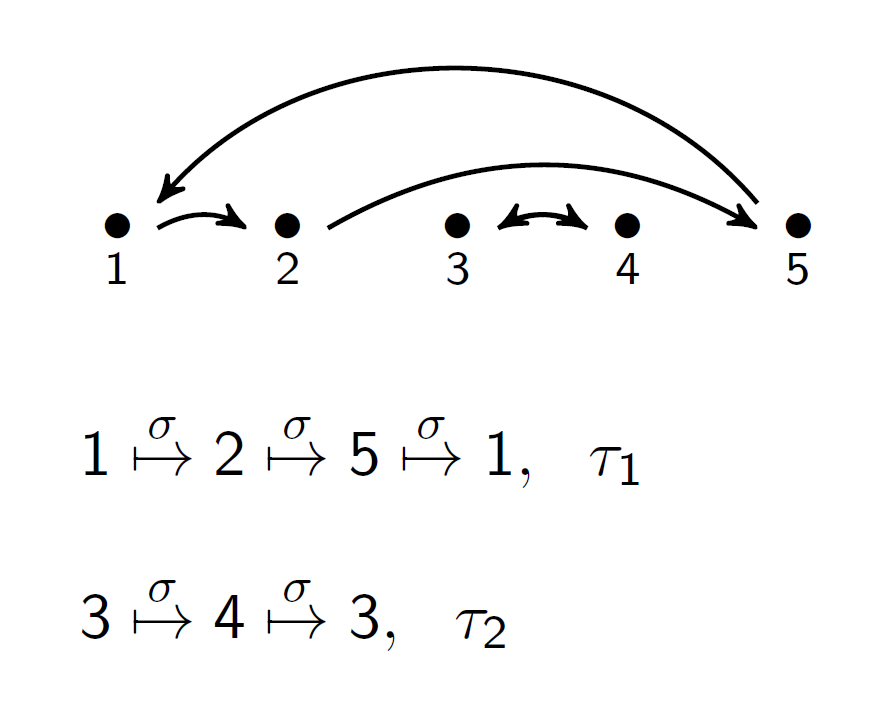
\includegraphics[scale=0.5]{Cycle.png}
    \caption{Example of Cycle}
\end{figure}
\end{center}
In the example of \textit{Figure 1}, $\sigma=\begin{pmatrix}
    1&2&3&4&5\\
    5&1&4&3&2
\end{pmatrix}$, $\sigma=\tau_1\circ\tau_2$, where $\tau_1=\begin{pmatrix}
    1&2&3&4&5\\
    5&1&3&4&2
\end{pmatrix}$, $\tau_2=\begin{pmatrix}
    1&2&3&4&5\\
    1&2&4&3&5
\end{pmatrix}$. $\tau_1$ is 3-cycle, $\tau_2$ is 2-cycle.
We could represent $\tau_1=(1\ 5\ 2)=(5\ 2\ 1)=(2\ 1\ 5)$, i.e.
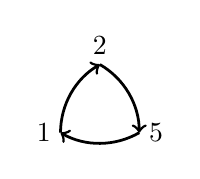
\begin{tikzpicture}[domain=0:3.25]
\draw[->,line width=1] (0.5,0.5*3^0.5) arc (60:0:0.5*2);
\draw[<-,line width=1] (0.5,0.5*3^0.5) arc (120:180:0.5*2);
\draw[<-,line width=1] (0,0) arc (240:300:0.5*2);
\node[left] at (0,0) {$1$};
\node[right] at (0.5*2,0) {$5$};
\node[above] at (0.5,0.5*3^0.5) {$2$};
\end{tikzpicture}
Similarly, we can represent $\tau_2=(3,4)=(4,3)$, i.e.
\begin{tikzpicture}[domain=0:3.25]
    \draw[<->](0,0)--(1,0) node[below] {$$};
    \node[left] at (0,0) {$3$};
    \node[right] at (1,0) {$4$};
\end{tikzpicture}\\
We can find that $\forall x\in \{1,2,3,4,5\}$, $\tau_1^{3}(x)=x, \tau_2^{2}(x)=x$, so we write $\tau_1$ as a \textbf{3-cycle} in $S_5$, $\tau_2$ as a \textbf{2-cycle} in $S_5$.\\

Given $k \geq 2$, a \textbf{k-cycle} in $S_n$ is a permutation $\sigma$ with the property that $\{1,...,n\}$ is the union of two disjoint subsets, $\{1,...,n\}=Y \cup Z $ and $Y \cap Z =\emptyset$, such that\\
1. $\sigma(x) = x$ for every $x \in Z$, and\\
2. $|Y| = k$, and for any$ x \in Y$,$Y = \{\sigma (x), \sigma^2(x), \sigma^3(x)... \sigma^k(x) = x\}$.\\

We say that $\sigma$ \textbf{cyclically permutes} the elements of $Y$ and \textbf{fixes} the elements of $Z$.\\
$\tau_1=(1\ 2\ 5)$ \textbf{cyclically permutes} the elements of $Y=\{1,2,5\}$ and \textbf{fixes} the elements of $Z=\{3,4\}$.\\
$\tau_2=(3\ 4)$ \textbf{cyclically permutes} the elements of $Y=\{3,4\}$ and \textbf{fixes} the elements of $Z=\{1,2,5\}$.\\


\subsection{Disjoint cycles}
Since the sets are cyclically permuted by $\tau_1, \tau_2$ (i.e.$Y$) are disjoint. We call the \textbf{disjoint cycle notation} $\sigma=\tau_1\circ\tau_2=(1\ 2\ 5)(3\ 4)$. (Commute the order is irrelevant)

\subsubsection{Theorem: Every permutation is a union of disjoint
cycles, uniquely.}
Given $\sigma\in S_n$, there exists a unique (possibly empty) set of pairwise disjoint cycles.
\begin{theorem}
Let $X$ be a finite set, the graph of permutation $\sigma\in S_X$ is a union of disjoint cycle.
\end{theorem}
\begin{proof}
Prove by induction:

If $|X|=1$, the graph is circle:
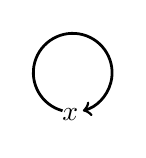
\begin{tikzpicture}[domain=-0.5:1]
    \draw[->,line width=1] (0.5,-0.65) arc (255:-75:0.5);
    \node[below] at (0.6,-0.5) {$x$};
\end{tikzpicture}

For $|X|>1$, let $i_1\in X$ and let $\mathcal{O}(i_1)=\{\sigma^r(i_1),r\geq 0\}=\{i_1,\sigma(i_1),\sigma^2(i_1),...\}$. $\mathcal{O}(i_1)$ is finite, and there is a smallest $r$ s.t. $\sigma^r(i_1)\in\{i_1,\sigma(i_1),\sigma^2(i_1),...,\sigma^{r-1}(i_1)\}$. Then $\sigma^r(i_1)=i_1$ because other elements already have a pre-change under $\sigma$.

Then $i_1 \rightarrow \sigma(i_1) \rightarrow \sigma^2(i_1)\rightarrow \cdots \rightarrow \sigma^{r-1}(i_1) \rightarrow	i_1$ is a cycle of length $r$.

For $j\notin \mathcal{O}(i_1), \sigma(j)\notin \mathcal{O}(i_1), \sigma^{-1}(j)\notin \mathcal{O}(i_1)$. Let $Y=X/\mathcal{O}(i_1)$ then $\sigma: Y \rightarrow	Y$ is a bijection. Then prove by induction.

\end{proof}

\begin{example}
$\sigma_1=(1\ 2\ 6\ 5)(3)(4)$, can be written by $\sigma_1=(1\ 2\ 6\ 5)$, $\sigma_2=(2\ 3\ 5\ 4)$
\end{example}
$\sigma_1 \circ \sigma_2=(1\ 2\ 6\ 5)\circ (2\ 3\ 5\ 4)$
\begin{equation}
    \begin{aligned}
        1 \stackrel{(2\ 3\ 5\ 4)}{\longrightarrow} 1 \stackrel{(1\ 2\ 6\ 5)}{\longrightarrow} 2\\
        2 \stackrel{(2\ 3\ 5\ 4)}{\longrightarrow} 3 \stackrel{(1\ 2\ 6\ 5)}{\longrightarrow} 3\\
        3 \stackrel{(2\ 3\ 5\ 4)}{\longrightarrow} 5 \stackrel{(1\ 2\ 6\ 5)}{\longrightarrow} 1\\
        4 \stackrel{(2\ 3\ 5\ 4)}{\longrightarrow} 2 \stackrel{(1\ 2\ 6\ 5)}{\longrightarrow} 6\\
        5 \stackrel{(2\ 3\ 5\ 4)}{\longrightarrow} 4 \stackrel{(1\ 2\ 6\ 5)}{\longrightarrow} 4\\
        6 \stackrel{(2\ 3\ 5\ 4)}{\longrightarrow} 6 \stackrel{(1\ 2\ 6\ 5)}{\longrightarrow} 5\\
    \end{aligned}
    \nonumber
\end{equation}
Then $\sigma_1 \circ \sigma_2=(1\ 2\ 3)\circ (4\ 6\ 5)$

$\sigma_2 \circ \sigma_1=(2\ 3\ 5\ 4)\circ (1\ 2\ 6\ 5)$
\begin{equation}
    \begin{aligned}
        1 \stackrel{(1\ 2\ 6\ 5)}{\longrightarrow} 2 \stackrel{(2\ 3\ 5\ 4)}{\longrightarrow} 3\\
        2 \stackrel{(1\ 2\ 6\ 5)}{\longrightarrow} 6 \stackrel{(2\ 3\ 5\ 4)}{\longrightarrow} 6\\
        3 \stackrel{(1\ 2\ 6\ 5)}{\longrightarrow} 3 \stackrel{(2\ 3\ 5\ 4)}{\longrightarrow} 5\\
        4 \stackrel{(1\ 2\ 6\ 5)}{\longrightarrow} 4 \stackrel{(2\ 3\ 5\ 4)}{\longrightarrow} 2\\
        5 \stackrel{(1\ 2\ 6\ 5)}{\longrightarrow} 1 \stackrel{(2\ 3\ 5\ 4)}{\longrightarrow} 1\\
        6 \stackrel{(1\ 2\ 6\ 5)}{\longrightarrow} 5 \stackrel{(2\ 3\ 5\ 4)}{\longrightarrow} 4\\
    \end{aligned}
    \nonumber
\end{equation}
Then $\sigma_2 \circ \sigma_1=(1\ 3\ 5)\circ (2\ 6\ 4)$

Note: $\sigma_1 \circ \sigma_2\neq\sigma_2 \circ \sigma_1$

\begin{example}[Exercise 1.3.2.]
    Consider $\sigma = (3\ 4\ 8)(5\ 7\ 6\ 9)$ and $\tau = (1\ 9\ 3\ 5)(2\ 7\ 4)$ in $S_9$ expressed in disjoint cycle
    notation. Compute $\sigma\circ\tau$ and $\tau\circ\sigma$ expressing both in disjoint cycle notation.
\end{example}

\begin{equation}
    \begin{aligned}
        &1 \rightarrow \sigma(\tau(1))=\sigma(9)=5;\ 
        2 \rightarrow \sigma(\tau(2))=\sigma(7)=6;\\
        &3 \rightarrow \sigma(\tau(3))=\sigma(5)=7;\ 
        4 \rightarrow \sigma(\tau(4))=\sigma(2)=2;\\
        &5 \rightarrow \sigma(\tau(5))=\sigma(1)=1;\ 
        6 \rightarrow \sigma(\tau(6))=\sigma(6)=9;\\
        &7 \rightarrow \sigma(\tau(7))=\sigma(4)=8;\ 
        8 \rightarrow \sigma(\tau(8))=\sigma(8)=3;\\
        &9 \rightarrow \sigma(\tau(9))=\sigma(3)=4;\\
        \Rightarrow	&\sigma\circ\tau=(1\ 5)(2\ 6\ 9\ 4)(3\ 7\ 8)
    \end{aligned}
    \nonumber
\end{equation}
\begin{equation}
    \begin{aligned}
        &1 \rightarrow \tau(\sigma(1))=\tau(1)=9;\ 
        2 \rightarrow \tau(\sigma(2))=\tau(2)=7;\\
        &3 \rightarrow \tau(\sigma(3))=\tau(4)=2;\ 
        4 \rightarrow \tau(\sigma(4))=\tau(8)=8;\\
        &5 \rightarrow \tau(\sigma(5))=\tau(7)=4;\ 
        6 \rightarrow \tau(\sigma(6))=\tau(9)=3;\\
        &7 \rightarrow \tau(\sigma(7))=\tau(6)=6;\ 
        8 \rightarrow \tau(\sigma(8))=\tau(3)=5;\\
        &9 \rightarrow \tau(\sigma(9))=\tau(5)=1;\\
        \Rightarrow	&\tau\circ\sigma=(1\ 9)(2\ 7\ 6\ 3)(4\ 8\ 5)
    \end{aligned}
    \nonumber
\end{equation}
\begin{example}
    Let $\sigma,\tau \in S_7$, given in disjoint cycle,
    notation by
    $\sigma = (1\ 5\ 4)(3\ 7),
    \tau = (1\ 3\ 2\ 6\ 4)$,
    Compute
    $\sigma^2 ,
    \sigma^{-1} ,
    \tau\circ \sigma$
\end{example}
\begin{equation}
    \begin{aligned}
        &\sigma^2=(1\ 4\ 5),&\sigma^{-1}=(4,5,1)(3,7),\\
        &1 \rightarrow	\tau(\sigma(1))=\tau(5)=5,
        &2 \rightarrow	\tau(\sigma(2))=\tau(2)=6,\\
        &3 \rightarrow	\tau(\sigma(3))=\tau(7)=7,
        &4 \rightarrow	\tau(\sigma(4))=\tau(1)=3,\\
        &5 \rightarrow	\tau(\sigma(5))=\tau(4)=1,
        &6 \rightarrow	\tau(\sigma(6))=\tau(6)=4,\\
        &7 \rightarrow	\tau(\sigma(7))=\tau(3)=2,\\
        \Rightarrow	& \tau\circ \sigma=(1,5)(2,6,4,3,7)
    \end{aligned}
    \nonumber
\end{equation}



\subsubsection{Cycle Structure}
\begin{enumerate}[$\bullet$]
    \item How many permutation $\sigma\in S_{12}$ has cycle structure $(1\ 2\ 3)(4\ 5\ 6)(7\ 8)(9\ 10)(11\ 12)$?
    $$\frac{12!}{3^22^3(2!)(3!)}$$
    $12!$: 每个位置的排列

    $3^2$: 每个长度3的cycle的每种情况会被重复计算3次

    $2^3$: 每个长度2的cycle的每种情况会被重复计算
    2次

    $(2!)$: 2个长度3的cycle具有不同位置的排列

    $(3!)$: 3个长度2的cycle具有不同位置的排列
    \item $(1\ 2\ 3)(4\ 5)(6)\in S_6$?
    $$\frac{6!}{3\times 2}=120$$
    \item General situation: $\sigma\in S_n$, $r_i$ category of length $i$, $i=1,2...$
    $$\frac{n!}{[1^{r_1}2^{r_2}3^{r_3}\cdots][(r_1!)(r_2!)(r_3!)\cdots]}$$
\end{enumerate}


\subsection{Transposition}
\begin{definition}
A \textbf{transposition} is a cycle of length 2: $\sigma=(i\ j)$.
\end{definition}

\subsubsection{Theorem: 每个permutation可以由若干个(可能不disjoint的)transposition表示}
\begin{theorem}
    Every permutation $\sigma$ of $X$ is a product of transposition. (the product is not unique)

    \textbf{Equivalent:} Given $n\geq2$, any $\sigma \in S_n$ can be expressed as a composition of 2-cycles.(not require disjoint)
\end{theorem}
\begin{proof}
    \quad\\

    Version 1:
    \begin{equation}
        \begin{aligned}
            (x_1\ x_{k})(x_1\ x_2,...\ x_{k-1}\ x_{k})&=(x_1\ x_2\ ...\ x_{k-1})\\
            (x_1\ x_2\ ...\ x_{k-1}\ x_{k})&=(x_1\ x_{k})(x_1,x_2\ ...\ x_{k-1})\\
            &=\mathbf{(x_1\ x_{k})(x_1\ x_{k-1})(x_1\ x_2\ ...\ x_{k-2})}\\
            &\dots\\
            &=\mathbf{(x_1\ x_{k})(x_1\ x_{k-1})(x_1\ x_{k-2})\dots(x_1\ x_2)}\\
        \end{aligned}
        \nonumber
    \end{equation}
    Version 2:
    \begin{equation}
        \begin{aligned}
            (x_1\ x_2,...\ x_{k-1}\ x_{k})(x_1\ x_{k})&=(x_2\ x_3\ ...\ x_{k})\\
            (x_1\ x_2\ ...\ x_{k-1}\ x_{k})&=(x_2\ x_3\ ...\ x_{k})(x_1\ x_{k})\\
            &\dots\\
            &=\mathbf{(x_{k-1}\ x_{k})(x_{k-2}\ x_{k})\dots(x_2\ x_{k})(x_1\ x_k)}\\
        \end{aligned}
        \nonumber
    \end{equation}
\end{proof}

\begin{claim}
Cycle of length $k$ can be written as a product of $k-1$ transpositions.
\end{claim}


\subsubsection{Sign of Permutation}
\begin{theorem}
Although the product of transposition of a permutation is not unique, the \underline{parity (odd or even) of the number of transposition} in a product is unique. We call it the \textbf{sign} of permutation.
\begin{equation}
    \begin{aligned}
        sign(\sigma)&=(-1)^{(\#\text{ even-length cycles in }\sigma)}\\
        &=(-1)^{(\#\text{ transpositions in }\sigma)}
    \end{aligned}
    \nonumber
\end{equation}
\end{theorem}

\begin{example}
\quad

$\sigma_1=(1\ 4\ 7\ 9)(2\ 8)(6\ 10)$: $N=3+1+1=5$ is odd.

$\sigma_2=(1\ 2\ 3\ 4\ 5)(6\ 7\ 8\ 9\ 10)$: $N=4+4=8$ is even
\end{example}

What happens to a permutation $\sigma$'s cycles if $\sigma \rightarrow (i\ j)\circ\sigma$?

1. $i$ and $j$ are not contained in $\sigma$.

2. $i$ and $j$ appear in the same cycle of $\sigma$.

3. $i$ and $j$ appear in disjoint cycles.

\begin{equation}
    \begin{aligned}
        (i\ j)\circ (i-- j\sim\sim)&=(i--)\circ(j\sim\sim)\\
        (i\ j)\circ(i--)\circ(j\sim\sim)&=(i-- j\sim\sim)
    \end{aligned}
    \nonumber
\end{equation}
\begin{proposition}
    $sign((i\ j)\circ\sigma)=-1\cdot sign(\sigma)$
\end{proposition}
\begin{proof}
\quad\\

Suppose $\sigma=(a_1\ a_2\ \cdots a_k\ b_1\ b_2\ \cdots b_l)$

Then $(a_1\ b_1)\circ\sigma=(a_1\ a_2\ \cdots a_k)(b_1\ b_2\ \cdots b_l)$
$$sign(\sigma)=\left\{\begin{matrix}
    +1&\text{ if $k+l$ is odd}\\
    -1&\text{ if $k+l$ is even}
\end{matrix}\right.$$
$$sign((a_1\ b_1)\circ\sigma)=\left\{\begin{matrix}
    -1&\text{ if $k+l$ is odd}\\
    +1&\text{ if $k+l$ is even}
\end{matrix}\right.$$

\end{proof}








\section{Integers}
\subsection{Proposition 1.4.1: Properties of integers $\mathbb{Z}$}
\begin{proposition}[Proposition 1.4.1.]
    The following hold in the integers $\mathbb{Z}$:
\end{proposition}
(i) \textit{Addition} and \textit{multiplication} are \textit{commutative} and \textit{associative} operations in $\mathbb{Z}$.\\
(ii) $0 \in \mathbb{Z}$ is an identity element for addition; that is, $\forall a \in \mathbb{Z}, 0 + a = a$.\\
(iii) Every $a \in \mathbb{Z}$ has an additive inverse, denoted $-a$ and given by $-a = (-1)a$, satisfying $a + (-a) = 0$.\\
(iv) $1 \in \mathbb{Z}$ is an identity element for multiplication; that is, for all $a \in \mathbb{Z}$, $1a = a.$\\
(v) The \textit{distributive} law holds: $\forall a,b,c \in \mathbb{Z}, a(b + c) = ab + ac$.\\
(vi) Both $\mathbb{N} = \{x \in Z | x \geq 0\}$ and $\mathbb{Z}_+ = \{x \in \mathbb{Z} | x > 0\}$ are $closed$ under $addition$ and $multiplication$.
That is, if $x$ and $y$ are in one of these sets, then $x + y$ and $xy$ are also in that set.\\
(vii) For any two nonzero integers $a,b\in\mathbb{Z}, |ab|\geq \max\{|a|,|b|\}$. Strict inequality holds if $|a| > 1$ and $|b| > 1$.\\

From this we get cancellation.
\begin{equation}
    \begin{aligned}
        ab=ac \Rightarrow	b=c \textit{ or } a=0
    \end{aligned}
    \nonumber
\end{equation}

\subsection{Definition: Divide}
Suppose $a,b\in\mathbb{Z},b\neq 0$, \underline{$b$ divides $a$} if $\exists m\in\mathbb{Z}$, so that $a=bm, b|a$. Otherwise, write $b \nmid a$.

\subsection{Proposition 1.4.2: properties of integer division}
\begin{proposition}[Proposition 1.4.2]
    $\forall a,b\in\mathbb{Z}$
\end{proposition}
(i) if $a\neq0$, then $a|0$\\
(ii) if $a|1$, then $a=\pm 1$\\
(iii) if $a|b\ \&\ b|a$, then $a=\pm b$\\
(iv) if $a|b\ \&\ b|c$, then $a|c$\\
(v) if $a|b\ \&\ a|c$, then $a|(mc+nb)\forall m,n\in\mathbb{Z}$\\

\subsection{Definitions: Prime, The Greatest common divisor $gcd(a,b)$}
$p > 1, p \in \mathbb{Z}$ is called
\underline{\textit{prime}} if the only divisors are
$\pm 1,\pm p$.

Given $a,b\in\mathbb{Z},a, b\neq 0$, the \underline{\textit{greatest common divisor}} of $a$ and $b$ is $c\in\mathbb{Z}, c>0$ s.t.

(1) $c|a$ and $c|b$; (2) if $d|a, d|b$, then $d|c$

The $c$ is unique, we write it $gcd(a,b)$.

\subsection{Euclidean Algorithm}
\begin{proposition}[Proposition 1.4.7(Euclidean Algorithm)]
    Given $a,b\in\mathbb{Z},b\neq 0$, then $\exists q,r\in \mathbb{Z}$ s.t. $a=qb+r, 0\leq r\leq |b|$.
\end{proposition}

\begin{example}[Exercise 1.4.3]
    For the pair $(a,b) = (130, 95)$, find $gcd(a, b)$ using the \textit{Euclidean Algorithm} and express it in the form $gcd(a,b) = sa + tb$ for $s, t \in Z$.
\end{example}
\begin{equation}
    \begin{aligned}
        &130=95+35;
        &95=2\times35+25\\
        &35=25+10;
        &25=2\times10+5\\
        &10=2\times5+0
    \end{aligned}
    \nonumber
\end{equation}
\begin{equation}
    \begin{aligned}
        5&=25-2\times10
        =25-2\times(35-25)
        =3\times25-2\times35=3\times(95-2\times35)-2\times35\\
        &=3\times95-8\times35=3\times95-8\times(130-95)=11\times95-8\times130
    \end{aligned}
    \nonumber
\end{equation}
\begin{equation}
    \begin{aligned}
        gcd(130,95)=gcd(95,35)=gcd(35,25)=gcd(25,10)=gcd(10,5)=gcd(5,0)=5
    \end{aligned}
    \nonumber
\end{equation}
We can also express it by matrix
\begin{center}
    \begin{tabular}{ccccc}
            \hline
            & $q$& $r$&$s$&$t$\\
            \hline
            -1&&130&1&0\\
            0&1&95&0&1\\
            1&2&35&1&-1\\
            2&1&25&-2&3\\
            3&2&10&3&-4\\
            4&2&5&-8&11\\
            \hline
    \end{tabular}
\end{center}
Hence $gcd(130,95)=5=-8\cdot130+11\cdot95$
\subsection{Proposition: $gcd(a,b)$ exists and is the smallest positive integer in the set $M=\{ma+nb|m,n\in\mathbb{Z}\}$}

\begin{theorem}
    $d = gcd(a, b)$ is of the form $sa + tb$
\end{theorem}
\begin{proof}

We may assume $0\leq a\leq b$

For $a=0$, $d=b=0\cdot a+1\cdot b$.

For $a>0$, let $b=q\cdot a+r$ with $0\leq r<a\leq b$. Then
\begin{equation}
    \begin{aligned}
        \{sa+tb:s,t\in \mathbb{Z}\}&=\{sa+t(q\cdot a+r):s,t\in \mathbb{Z}\}=\{tr+ua: t,u\in \mathbb{Z}\}\\
        &=\dots \{x\cdot 0+y\cdot d: x,y\in \mathbb{Z}\}=\{...,-2d,-d,0,d,2d,...\}
    \end{aligned}
    \nonumber
\end{equation}
\end{proof}

\begin{proposition}[第二种表示,第二种证明]
    $\forall a,b\in\mathbb{Z}$, not both 0, $gcd(a,b)$ exists and is the smallest positive integer in the set $M=\{ma+nb|m,n\in\mathbb{Z}\}$. i.e. $\exists m_0,n_0\in\mathbb{Z}$ s.t. $gcd(a,b)=m_0a+n_0b$.
\end{proposition}

\begin{proof}

Let $c$ be the smallest positive integer in the set $M=\{ma+nb|m,n\in\mathbb{Z}\}$. $c=m_0 a+n_0 b>0$.

Let $d=ma+nb\in M$, $d=qc+r$ where $0\leq r<c$ (by Euclidean Algorithm).
$$r=d-qc=(m-qm_0)a+(n-qn_0)b\in M$$
Since $c$ is the smallest integer in $M$ and $r\in[0,c)$, so $r=0$. $\Rightarrow d=qc$. So $c|d$.

$a=1a+0b\in M\Rightarrow c|a$, $b=0a+1b\in M\Rightarrow c|b$.

If $t|a,t|b$ then $t|m_0 a+n_0 b \text{ i.e. } t|c$. $\Rightarrow c=gcd(a,b)$.
\end{proof}

\subsection{Well-Ordering Principle (Least Integer Axiom)}
There is a smallest integer in every nonempty subset $S$ of the natural numbers $\mathbb{N}=\{0,1,2,...\}$

\subsection{Proposition 1.4.10: $gcd(b,c)$, $b|ac$ $\Rightarrow$ $b|a$}
\begin{proposition}[Proposition 1.4.10]
    Suppose $a,b,c\in\mathbb{Z}$. If $b,c$ are \textit{relatively prime} i.e. $gcd(b,c)=1$ and $b|ac$, then $b|a$.
\end{proposition}
\begin{proof}
$gcd(b,c)=1\Rightarrow\ \exists m,n\in\mathbb{Z}$ s.t. $1=mb+nc \Rightarrow a=amb+anc$. Since $b|nac, b|amb\Rightarrow b|a$.
\end{proof}
\subsubsection{Corollary: $p|ab$ $\Rightarrow	$ $p|a$ or $p|b$}
\begin{corollary}[Corollary of Prop 1.4.10]
    $a,b,p\in\mathbb{Z}, p>1$ prime. If $p|ab$, then $p|a$ or $p|b$.
\end{corollary}
\begin{proof}
If $p|b$, done. Otherwise, $gcd(p,b)=1$. By Prop 1.4.10, $p|a$.
\end{proof}


\subsection{Fundamental Theorem of Arithmetic: Any integer
$a \geq 2$ has a unique prime factorization}

\subsubsection{Existence}
\begin{lemma}
    Any integer $a \geq 2$ is either a prime or a product of primes.
\end{lemma}
\begin{proof}
    Set $S\subset \mathbb{N}$ be the set of all $n$ without the given property.
    
    Assume that $S$ in nonempty and $m$ is the least element in $S$.

    Since $m$ is not a prime, it can be written as $m=ab$ with $1<a,b<m$. Since $m$ is the least element in $S$, $a,b\notin S$. Then $m$ is a product of primes. Contradiction. Thus, $S=\emptyset$.
\end{proof}

\subsubsection{Uniqueness}
\begin{theorem}[Fundamental Theorem of Arithmetic]
\end{theorem}
Any integer
$a > 1$ has a unique prime factorization:
$a=p_1^{k_1}\cdot p_2^{k_2}\cdot...p_n^{k_n}$ where $p_i > 1$ is prime, $k_i\in\mathbb{Z}_+,\forall i=1,...,n, p_i\neq p_j, \forall i\neq j$.
\begin{proof}
\quad

\begin{enumerate}[a)]
    \item Existence: (Previous Lemma)
    \item Uniqueness: \begin{enumerate}[1)]
        \item Method 1:
        
        Suppose $a=p_1^{n_1}\cdot p_2^{n_2}\cdot...p_k^{n_k}=q_1^{r_1}\cdot q_2^{r_2}\cdot...q_j^{r_j}$. Where $p_1>p_2>...>p_k, q_1>q_2>...>q_j, n_i,r_i\geq 1$.

        $p_1|a\Rightarrow \exists\ q_i\ s.t.\ p_1|q_i$. Similarly, $\exists\ q_i\ s.t.\ q_1|p_{i'}$.
        
        $q_1\leq p_{i'}\leq p_1\leq q_i\Rightarrow q_1= p_{i'}= p_1= q_i$
        
        We can also know $n_1=r_1$, otherwise we would have two prime factorization of the quotient where the largest primes are different by dividing $p_1^{\min\{n_1,r_1\}}$.
        
        Then we can get $b=p_2^{n_2}\cdot...p_k^{n_k}=q_2^{r_2}\cdot...q_j^{r_j}$. Then prove it by induction.

        \item Method 2:
        
        Suppose $a=p_1\cdot p_2\cdot...p_k=q_1\cdot q_2\cdot...q_t$. For a $p_i$, there must exist a $q_j$ s.t. $p_i=q_j$:

        Assume that $p_i\neq q_t$, $gcd(p_i,q_t)=1$. Then $\exists a,b$ such that $1=ap_i+bq_t$. Multiplying both sides by $q_1\cdot q_2\cdot...q_{t-1}$: $$q_1\cdot q_2\cdot...q_{t-1}=ap_iq_1\cdot q_2\cdot...q_{t-1}+bq_1\cdot q_2\cdot...q_t$$
        Since $p_i|q_1\cdot q_2\cdot...q_t$, we can conclude that $p_i|(ap_iq_1\cdot q_2\cdot...q_{t-1}+bq_1\cdot q_2\cdot...q_t)$ $$\text{i.e. } p_i|q_1\cdot q_2\cdot...q_{t-1}\text{ if }p_i\neq q_t$$
        Then prove by induction.
    \end{enumerate}
\end{enumerate}
\end{proof}

\section{Modular arithmetic}
\subsection{Congruences}
\subsubsection{Congruent modulo $m$: $a\equiv b \text{ mod }m$}
Given $m\in\mathbb{Z}_+$, define a relation on $\mathbb{Z}$: \underline{\textbf{congruence modulo $m$}}
\begin{equation}
    \begin{aligned}
        a\equiv b \text{ mod }m\text{, if } m|(a-b)
    \end{aligned}
    \nonumber
\end{equation}
Read as "$a$ is congruent to $b$ mod $n$"; Notation: $a\equiv b$ mod $m$.

Equivalent to: $a,b$ have the same remainder after division by $m$.
\subsubsection{Proposition: For fixed $m\geq 2$, the relation "$a\sim b$ $\Leftrightarrow$ $a\equiv b$ mod $m$" is an \underline{equivalence relation}}
\begin{proposition}[Proposition 1.5.1]
    For fixed $m\geq 2$, the relation "$a\sim b$ $\Leftrightarrow$ $a\equiv b$ mod $m$" is an \underline{equivalence relation}
\end{proposition}
\begin{proof}
\quad

\begin{enumerate}[1)]
    \item \underline{Reflexive}: $\forall a\in\mathbb{Z}, m|0=(a-a)$, so $a\equiv a \text{ mod }m$ i.e. $a\sim a$.
    \item \underline{Symmetric}: $\forall a,b\in\mathbb{Z}$, $a\equiv b \text{ mod }m$, then $m|(a-b)\Rightarrow m|(b-a)$$\Rightarrow b\equiv a \text{ mod }m$. i.e. $a\sim b \Rightarrow b\sim a$.
    \item \underline{Transitive}: $\forall a,b,c\in\mathbb{Z}$, $a\equiv b \text{ mod }m$, $b\equiv c \text{ mod }m$. Then $m|(a-b), m|(b-c)$ $\Rightarrow m|(a-b)+(b-c)=(a-c)\Rightarrow a\equiv c \text{ mod }m$.
\end{enumerate}
\end{proof}

\subsubsection{Theorem: the equivalence relation "$a\sim b$ $\Leftrightarrow$ $a\equiv b$ mod $m$" partitions the integers into $m$ disjoint sets $\Omega_i=\{a|a\sim i\},i=0,1,...,m-1$}
\begin{theorem}
    the equivalence relation "$a\sim b$ $\Leftrightarrow$ $a\equiv b$ mod $m$" partitions the integers into $m$ disjoint sets $\Omega_i=\{a|a\sim i\},i=0,1,...,m-1$
\end{theorem}
\begin{proof}
    Prove any $a\in \mathbb{Z}$ belongs to a unique $\Omega_i$.

    \begin{enumerate}[a)]
        \item Existence: Division Algorithm $\Rightarrow$ $a=qm+r$, $0\leq r<m$. $a\in\Omega_r$.
        \item Uniqueness: Assume $a$ in two sets, $a\in\Omega_r\cap \Omega_{r^1}$, $0\leq r^1<r<m$.
        
        Then $m|a-r$ and $m|a-r^1$ $\Rightarrow$ $m|r-r^1$, which is impossible because $0<r-r^1<m$. Contradiction.
    \end{enumerate}
\end{proof}

\subsubsection{Proposition: Addition and Mutiplication of Congruences}
\begin{proposition}
    Fix integer $m\geq 2$. If $a\equiv r \text{ mod }m$ and $b\equiv s \text{ mod }m$, then $a+b\equiv r+s \text{ mod }m$ and $ab\equiv rs \text{ mod }m$
\end{proposition}
\begin{proof}
\quad

\begin{enumerate}[a)]
    \item Addition: $m|(a-r), m|(b-s)\Rightarrow m|(a-c)+(b-d)\Rightarrow m|(a+b)-(c-d)$.
    \item Mutiplication: $m|(a-r)b+r(b-s)\Rightarrow m|ab-rs$.
\end{enumerate}
\end{proof}

\subsection{Solving Linear Equations on Modular $m$}
\subsubsection{Theorm: unique solution of $aX\equiv b \text{ mod }m$ if $gcd(a,m)=1$}
\begin{theorem}
If $gcd(a,m)=1$, then $\forall b\in \mathbb{Z}$ the congruence $aX\equiv b \text{ mod }m$ has a unique solution.
\end{theorem}
\begin{proof}
\quad

\begin{enumerate}[1)]
    \item Existence: Since $gcd(a,m)=1$, $\exists s,t$ such that
    \begin{equation}
        \begin{aligned}
        1&=sa+tm\\
        (\text{Version 1})&\\
        &\text{(Mutiplying $X$)}\\
        X&=saX+tmX\\
        aX\equiv b \text{ mod }m &\Leftrightarrow aX=km+b\\
        &\Leftrightarrow X=s(km+b)+b\\
        &\Leftrightarrow X\equiv sb \text{ mod }m\\
        (\text{Version 2})&\\
        &\text{(Mutiplying $s$)}\\
        saX&\equiv sb \text{ mod }m\\
        (1-tm)X&\equiv sb \text{ mod }m\\
        X&\equiv sb \text{ mod }m\\
        \end{aligned}
        \nonumber
    \end{equation}
    $X\equiv sb \text{ mod }m$ is the solution to $aX\equiv b \text{ mod }m$.
    \item Uniqueness: Assume $x,y$ are two solutions, $$ax\equiv b \text{ mod },ay\equiv b \text{ mod } m\Rightarrow	a(x-y)\equiv 0 \text{ mod }m$$
    Since $gcd(a,m)=1,\ m|(x-y)\Rightarrow x=y,\ (x,y\in\{0,1,...,m-1\})$
\end{enumerate}
\begin{example}
Solve $3X\equiv 5 \text{ mod }11$.
\end{example}
$gcd(3,11)=1$, $1=4*3-1*11$, 
\begin{equation}
    \begin{aligned}
        X&\equiv 4*5\\
        X&\equiv 9
    \end{aligned}
    \nonumber
\end{equation}

\end{proof}

\subsection{Chinese Remaindar Theorem (CRT): unique solution for $x$ modulo $mn$}
\begin{theorem}[Chinese Remaindar Theorem (CRT)]
\quad

If $gcd(m,n)=1$. Then $\left\{\begin{matrix}
    x\equiv r \text{ mod }m& (1)\\
    x\equiv s \text{ mod }n& (2)
\end{matrix}\right.$ have a unique solution for $x$ modulo $mn$.
\end{theorem}
\begin{proof}
\quad\\
(1) $\Rightarrow x=km+r$ for some $k\in \mathbb{Z}$.

\begin{equation}
    \begin{aligned}
        \text{substitute (2) }&\Rightarrow	km+r\equiv s \text{ mod }n\\ &\Leftrightarrow	mk\equiv s-r \text{ mod }n\quad (3)
    \end{aligned}
    \nonumber
\end{equation}
According to previous theorem, $gcd(m,n)=1$, (3) has a \textbf{unique} solution.

We say $k\equiv t \text{ mod }n$, $k=ln+t$ for some $l\in \mathbb{Z}$

$\Rightarrow x=(ln+t)m+r=lnm+tm+r$, where $tm+r$ is the unique solution to $x$ modulo $mn$.
\end{proof}

\begin{example}(Similar to CRT)
Find the smallest integer $x$ such that $$x\equiv 1 \text{ mod }11\text{ and }x\equiv  9\text{ mod }13$$
\end{example}
$gcd(11,13)=1$ and $1=6*11-5*13$

Write $x=11k+1$. Substitute in $x\equiv 9 \text{ mod }13$:
\begin{equation}
    \begin{aligned}
        11k&\equiv 8 \text{ mod }13\\
        6*11k&\equiv 6*8\equiv 9 \text{ mod }13\\
        (1+5*13)k&\equiv 9 \text{ mod }13\\
        k&\equiv 9 \text{ mod }13\\
    \end{aligned}
    \nonumber
\end{equation}
Then $x=11k+1=100$.

\subsection{Congruence Classes: $[a]_n=\{a+kn|k\in\mathbb{Z} \}$}
将给定$n$,相同余数的数分为一组\\
Fix $n\in\mathbb{Z}_+$, we call $[a]_{n}=[a]$ the \underline{\textbf{congruence class}} of a modulo n.
\begin{equation}
    \begin{aligned}
        [a] = \{b \in \mathbb{Z}|b\equiv a \textit{ mod }n\}=\{a+kn|k\in\mathbb{Z} \}
    \end{aligned}
    \nonumber
\end{equation}

\subsubsection{Set of congruence classes of mod $n$: $\mathbb{Z}_n = \{[a]_n|a \in \mathbb{Z}\}=\{[0],[1],...,[n-1]\}$}
The set of \textit{congruence classes} of mod $n$ is denoted $\mathbb{Z}_n = \{[a]_n|a \in \mathbb{Z}\}$
\begin{proposition}[Proposition 1.5.2.]
For any $n\geq 1$ there are exactly $n$ congruences classes modulo $n$, which we may write as
\begin{equation}
    \begin{aligned}
        \mathbb{Z}_n = \{[0],[1],...,[n-1]\}
    \end{aligned}
    \nonumber
\end{equation}
\end{proposition}
\begin{proof}
\quad\\
For any $a\in\mathbb{Z}$. By Euclidean algorithm, $a=qn+r$, $q,r\in\mathbb{Z}$, $0\leq r<n\Rightarrow a\in[r]$. So, $\mathbb{Z}_n = \{[0],[1],...,[n-1]\}$.\\
When $0\leq a<b\leq n-1$, $n\nmid(b-a)$, so $[a]\neq [b]$ the $n$ congruence classes listed are all distinct. Hence, there are exactly $n$ congruence classes.
\end{proof}
\subsubsection{Proposition 1.5.5: Addition and Multiplication on Congruence Classes}
Fix $n\in\mathbb{Z}$, we define addition$+$ and multiplication$\cdot$ on $\mathbb{Z}_n$:
\begin{equation}
    \begin{aligned}
        &[a]+[b]=[a+b]=\{a+b+(k+j)n|k,j\in\mathbb{Z}\}\\
        &[a]\cdot [b]=[ab]=\{ab+(aj+bk+kjn)n|k,j\in\mathbb{Z} \}
    \end{aligned}
    \nonumber
\end{equation}
This is well defined, follows Lemma 1.5.3.
\begin{proposition}[Proposition 1.5.5.]
    Let $a,b,c,d,n\in\mathbb{Z}, n\geq 1$, then\\
    (i) Addition and multiplication are commutative and associative operations in $\mathbb{Z}_n$.\\
    (ii) $[a] + [0] = [a]$.\\(iii) $[-a] + [a] = [0]$.\\(iv) $[1][a] = [a]$.\\(v) $[a]([b] + [c]) = [a][b] + [a][c]$.
\end{proposition}
\begin{proof}
\quad\\

\end{proof}
\subsubsection{Units(i.e. invertible) in Congruence Classes}
将与$n$互质的数分为一组\\
Say $[a] \in \mathbb{Z}_n$ is a \textbf{unit} or is \textbf{invertible} if $\exists [b] \in \mathbb{Z}_n$ so that $[a][b] = [1]$.
\subsubsection{Proposition 1.5.6: Set of units in congruence classes: $\mathbb{Z}_n^{\times}=\{[a]\in\mathbb{Z}_n|[a] \textit{ is a unit}\}=\{[a]\in\mathbb{Z}_n|gcd(a,n)=1\}$}
The set of \textbf{invertible} elements in $\mathbb{Z}_n$ will be denoted $\mathbb{Z}_n^{\times}=\{[a]\in\mathbb{Z}_n|[a] \textit{ is a unit}\}$.
\begin{proposition}[Proposition 1.5.6.]
For all $n\geq 1$, we have $\mathbb{Z}_n^{\times}=\{[a]\in\mathbb{Z}_n|gcd(a,n)=1\}$.
\end{proposition}
\begin{proof}
    \quad\\
    By Proposition 1.4.8, we know there exists $b,c$ s.t. $ab+cn=1$. So, $ab \equiv 1 \textit{ mod }n$, $[1]=[ab]=[a][b]$. So, $\{[a]\in\mathbb{Z}_n|gcd(a,n)=1\}\subset \mathbb{Z}_n^{\times}$\\
    $[a] \textit{ is a unit}\Rightarrow $$\exists [b] \in \mathbb{Z}_n$ so that $[a][b] =[ab]= [1]\Rightarrow ab=1+kn, k\in \mathbb{Z}\Rightarrow ab-kn=1, k\in \mathbb{Z} \Rightarrow gcd(a,n)=1$. So, $\mathbb{Z}_n^{\times}\subset \{[a]\in\mathbb{Z}_n|gcd(a,n)=1\}$.
\end{proof}
\begin{note}
Inverse of $[a]$ is unique, i.e. $[b]=[a]^{-1}$ is unique.
\end{note}
$[a][b]=1, [a][b']=1\Rightarrow [b]=[b][1]=[b][a][b']=[b']$

\subsubsection{Corollary 1.5.7: if $p$ is prime, $\varphi(p)=\mathbb{Z}_p^{\times}=\{[1],[2],...,[p-1] \}$}
\begin{corollary}[Corollary 1.5.7]
If $p\geq2$ is prime, $\mathbb{Z}_p^{\times}=\{[1],[2],...,[p-1] \}$.
\end{corollary}
\subsection{\underline{Euler phi-function}: $\varphi(n)=|\mathbb{Z}_n^{\times}|$}
\underline{Euler phi-function}: $\varphi(n)=|\mathbb{Z}_n^{\times}|$.\\
$p$ prime, $\varphi(p)=p-1$.\\

\subsubsection{$m|n$, $\pi_{m,n}([a]_n)=[a]_m$}
\begin{example}[Exercise 1.5.4]
    If $m|n$, we can define $\pi_{m,n}:\mathbb{Z}_n\rightarrow\mathbb{Z}_m$ by $\pi_{m,n}([a]_n)=[a]_m$. Prove it is well-defined.
\end{example}
\begin{proof}
\quad\\
We write $[a]_n=[c]_n$, verify that $[a]_m=[c]_m$.\\
Since $m|n$, there exists $k\in\mathbb{Z}$ s.t. $n=km$.\\
$[a]_n=[c]_n\Rightarrow \exists j\in\mathbb{Z}$ s.t. $c=a+jn$.\\
$[c]_m=[a+jn]_m=[a+jkm]_m=[a]_m$
\end{proof}

\subsection{Theorem 1.5.8(Chinese Remainder Theorem): $n=mk,gcd(m,k)=1$, $F([a]_n)=(\pi_{m,n}([a]_n),\pi_{k,n}([a]_n))=([a]_m,[a]_k)$}
\begin{theorem}[Theorem 1.5.8(Chinese Remainder Theorem)]
If $m,n,k>0,n=mk,gcd(m,k)=1$, then $F:\mathbb{Z}_n\rightarrow\mathbb{Z}_m\times\mathbb{Z}_k$ which is given by $F([a]_n)=(\pi_{m,n}([a]_n),\pi_{k,n}([a]_n))=([a]_m,[a]_k)$, then $F$ is a bijection.
\end{theorem}
\begin{proof}
\quad\\
(1)Injective: $F([a]_n)=F([b]_n)\Rightarrow [a]_m=[b]_m,[a]_k=[b]_k$ i.e. $a\equiv b \textit{ mod }m,a\equiv b \textit{ mod }n$. $\exists i,j\in\mathbb{Z}$ s.t. $b=a+im=a+jk\Rightarrow k|im$. Since $gcd(m,k)=1$, $k|i\Rightarrow n=mk|im$. Then $[b]_n=[a]_n+[im]_n=[a]_n$.\\
(2)Surjective: prove $\forall u,v\in\mathbb{Z}$, $\exists a\mathbb{Z}$ s.t. $[a]_m=[u]_m,[a]_k=[v]_k$.\\
Since $gcd(m,k)=1$, $\exists s,t\in \mathbb{Z}$ so that $1=sm+tk$. \\
Let $a=(1-tk)u+(1-sm)v$, $[a]_m=[(u-v)sm+v]_m=[v]_m$, $[a]_k=[(v-u)tk+u]_k=[u]_k$.
\end{proof}
\begin{note}
    $F([a]_n[b]_n)=F([ab]_n)=([ab]_m,[ab]_k)=([a]_m[b]_m,[a]_k[b]_k)$
\end{note}
Since $F$ is a bijection, $[ab]_n=[1]_n$ iff $([a]_m[b]_m,[a]_k[b]_k)=([1]_m,[1]_k)$.
\subsubsection{Proposition 1.5.9+Corollary 1.5.10: $m,n,k>0,n=mk,gcd(m,k)=1$, then $F(\mathbb{Z}_n^{\times})=\mathbb{Z}_m^{\times}\times\mathbb{Z}_k^{\times}$, then $\varphi(n)=\varphi(m)\varphi(k)$}
\begin{proposition}[Proposition 1.5.9+Corollary 1.5.10]
    If $m,n,k>0,n=mk,gcd(m,k)=1$, then $F(\mathbb{Z}_n^{\times})=\mathbb{Z}_m^{\times}\times\mathbb{Z}_k^{\times}$, then $\varphi(n)=\varphi(m)\varphi(k)$.
\end{proposition}

\subsection{prime factorization: $n=p_1^{r_1}...p_k^{r_k}$, then $\varphi(n)=(p_1-1)p_1^{r_1-1}...(p_k-1)p_k^{r_k-1}$}
\begin{proposition}
If $n\in\mathbb{Z}$ is positive integre with prime factorization $n=p_1^{r_1}...p_k^{r_k}$, then $\varphi(n)=(p_1-1)p_1^{r_1-1}...(p_k-1)p_k^{r_k-1}$
\end{proposition}
\begin{proof}
\quad\\
$\mathbb{Z}_{p^r}=\{[0],[1],...,[p^r-1]\}$, the number of multiples of $p$ is $\frac{p^r}{p}=p^{r-1}$. Then $\varphi(p^r)=|\mathbb{Z}_{p^r}^{\times}|=p^r-p^{r-1}=(p-1)p^{r-1}$. So,
\begin{equation}
    \begin{aligned}
        \varphi(n)=\varphi(p_1^{r_1})...\varphi(p_k^{r_k})=(p_1-1)p_1^{r_1-1}...(p_k-1)p_k^{r_k-1}
    \end{aligned}
    \nonumber
\end{equation}
\end{proof}
\section{Complex numbers}
$\mathbb{C}=\{a+bi | a,b\in\mathbb{R}\}$, $\mathbb{R}=\{a+0i | a\in\mathbb{R}\}\subset \mathbb{C}$\\
Addition $\&$ multiplication
\begin{equation}
    \begin{aligned}
        (a + bi) + (c + di) &= (a + c) + (b + d)i\\
        (a + bi )(c + di) &= ac + bci + adi + bdi^2\\
        &= (ac-bd) + (bc + ad)i
    \end{aligned}
    \nonumber
\end{equation}
\textbf{\underline{Complex conjugation}}: $z = a + bi , \bar{z} = a - bi$, $\overline{zw}=\bar{z}\bar{w}$\\
\textbf{\underline{Absolute value}}: $|z| = \sqrt{a^2+b^2}$, $|z|^2=z\bar{z}$\\
\textbf{\underline{Additive inverse}}: $-z=-a-bi$\\
\textbf{\underline{Multiplicative inverse}}: $z^{-1}=\frac{1}{z}=\frac{1}{a+bi}=\frac{a-bi}{a^2+b^2}=\frac{\bar{z}}{|z|^2}$\\
\begin{equation}
    \begin{aligned}
        z\in\mathbb{C}, &\overline{z+\bar{z}}=\bar{z}+\bar{\bar{z}}=z+\bar{z}\\
        \textit{Real part: }&Re(z)=\frac{z+\bar{z}}{2}\\
        \textit{Imaginary part: }&Im(z)=\frac{z-\bar{z}}{2i}\\
    \end{aligned}
    \nonumber
\end{equation}

\subsection{Geometric Meaning of Addition and Multiplication}
\underline{Addition}: parallelogram law
\begin{center}\begin{figure}[htbp]
    \centering
    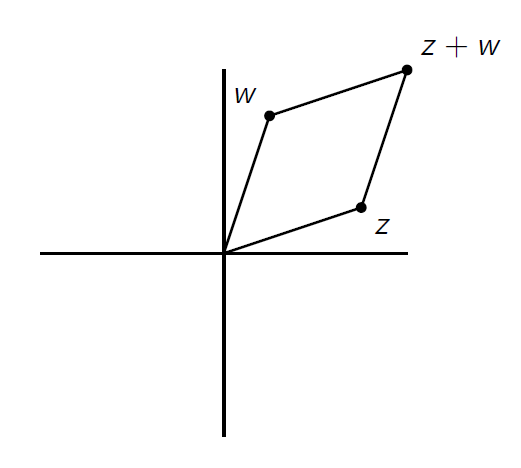
\includegraphics[scale=0.7]{Complex addition.png}
\end{figure}\end{center}
\underline{Multiplication}:
\begin{equation}
    \begin{aligned}
        z&=a+bi\neq0\\
        &=r \cos\theta+r \sin\theta i\\
        &=r (\cos\theta+i\sin\theta)\\
        |z|^2&=a^2+b^2=r^2
    \end{aligned}
    \nonumber
\end{equation}
\begin{equation}
    \begin{aligned}
        z=&r (\cos\theta+i\sin\theta)\\
        w=&s (\cos\phi+i\sin\phi)\\
        zw=&rs[\cos\theta\cos\phi-\sin\theta\sin\phi+i(\cos\theta\sin\phi+\cos\phi\sin\theta)]\\
        =&rs[cos(\theta+\phi)+i\sin(\theta+\phi)]\\
        =&|z||w|[cos(\theta+\phi)+i\sin(\theta+\phi)]
    \end{aligned}
    \nonumber
\end{equation}
\begin{center}\begin{figure}[htbp]
    \centering
    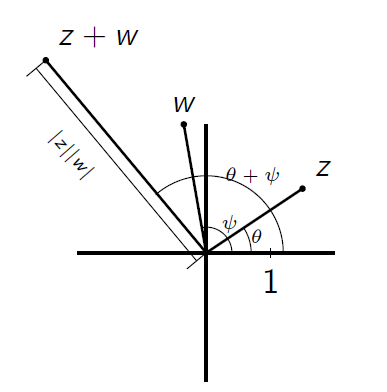
\includegraphics[scale=0.8]{Complex multiplication.png}
\end{figure}\end{center}
We will write,
\begin{equation}
    \begin{aligned}
        &\cos \theta+i\sin\theta=e^{i\theta}\\
        &e^{i\theta}e^{i\phi}=e^{i(\theta+\phi)}\\
        &z=|z|e^{i\theta}
    \end{aligned}
    \nonumber
\end{equation}
\subsection{Theorem 2.1.1: $f(x)=a_0+a_1x+...+a_nx^n$ with coefficients $a_0,a_1,...,a_n\in\mathbb{C}$. Then $f$ has a \underline{root} in $\mathbb{C}$: $\exists \alpha\in\mathbb{C}$ s.t. $f(\alpha)=0$}
\begin{theorem}[Theorem 2.1.1]
Supose a nonconstant polynomial $f(x)=a_0+a_1x+...+a_nx^n$ with coefficients $a_0,a_1,...,a_n\in\mathbb{C}$. Then $f$ has a \underline{root} in $\mathbb{C}$: $\exists \alpha\in\mathbb{C}$ s.t. $f(\alpha)=0$.
\end{theorem}
\subsubsection{Corollary 2.1.2: $f(x)=a_n\prod_{i=1}^n(x-k_i)=a_n(x-k_1)(x-k_2)...(x-k_n)$, where $k_1,k_2,...,k_n$ are roots of $f(x)$}
\begin{corollary}[Corollary 2.1.2]
    Every nonconstant polynomial with coefficients $a_0,a_1,...,a_n\in\mathbb{C}$ can be factored as $f(x)=a_n\prod_{i=1}^n(x-k_i)=a_n(x-k_1)(x-k_2)...(x-k_n)$, where $k_1,k_2,...,k_n$ are roots of $f(x)$.
\end{corollary}
\subsubsection{Corollary 2.1.3: $a_i\in \mathbb{R}$, $f$ can be expresses as a product of linear and quadratic polynomials}
\begin{corollary}[Corollary 2.1.3]
    If $f (x) = a_0 + a_1x + ... + a_nx^n$ is a nonconstant
    polynomial $a_0, a_1, ..., a_n \in \mathbb{R}, a_n \neq 0$.
    Then $f$ can be expresses as a product of linear and quadratic polynomials.
\end{corollary}
这里$a_0, a_1, ..., a_n$是实数!
\begin{proof}
\quad\\
(1)Obviously, the corollary holds at $n=1$ and $n=2$.\\
(2)Suppose the corollary holds for all situations that $n<k$.\\
When $n=k$, $f (x) = a_0 + a_1x + ... + a_kx^k, a_k\neq 0$.\\
By F.T.A., $f$ has a root $\alpha$ in $\mathbb{C}$.\\
If $\alpha\in\mathbb{R}$, long division $f(x)=q(x)(x-\alpha)$. $q$ has real coefficients, $\textit{degree of }q=k-1$. Since the corollary holds at $n=k-1$, $q(x)$ is a product of linear and quadratics. Then, the corollary also holds at $n=k$.\\
If $\alpha\notin\mathbb{R}$
\begin{equation}
    \begin{aligned}
        &0=f(\alpha)=a_0+a_1\alpha+...+a_k\alpha^k\\
        &0=\overline{f(\alpha)}={a_0}+{a_1}\bar{\alpha}+...+{a_n}\bar{\alpha}^n=f(\bar{\alpha})
    \end{aligned}
    \nonumber
\end{equation}
Since $\bar{\alpha}\neq\alpha$, $(x-\alpha)(x-\bar{\alpha})|f$.\\
$(x-\alpha)(x-\bar{\alpha})=x^2-(\alpha+\bar{\alpha})x+|\alpha|^2$ is a polynomial with coefficients in $\mathbb{R}$. So $f(x)=q(x)(x^2-(\alpha+\bar{\alpha})x+|\alpha|^2)$, $q$ has real coefficients with degree $k-2$. The corollary also holds at $n=k-2$, $q(x)$ is a product of linear and quadratics. Then, the corollary also holds at $n=k$.\\
\end{proof}

\section{Field $(\mathbb{F}, +, \cdot)$ (close, associative, commutative, distributive(M over A), identity $\&$ inverse(M,A))}
\textbf{\underline{Definition}}: A \underline{field} is a nonempty set $\mathbb{F}$ with two operations:\\
1. \underline{addition}, written $a+b, \forall a,b\in\mathbb{F}$; \\
2. \underline{multiplication}, written $a\cdot b=ab, \forall a,b\in\mathbb{F}$.\\
such that:\\
(i) \textit{addition} and \textit{multiplication} are \underline{associative} and \underline{commutative}\\
(ii) \textit{multiplication} \underline{distributes} over \textit{addition}: $a(b+c)=ab+ac, \forall a,b,c\in\mathbb{F}$\\
(iii) $\exists$ an \underline{additive identity} $0\in \mathbb{F}$ s.t. $0+a=a, \forall a\in \mathbb{F}$.\\
(iv)$\forall a\in\mathbb{F}$, $\exists$ an \underline{additive inverse} $-a$ s.t. $a+(-a)=0, \forall a\in\mathbb{F}$.\\
(v) $\exists$ a \underline{multiplicative identity}: $1\in\mathbb{F}$ s.t. $1a=a, \forall a\in\mathbb{F}, 1\neq 0$.\\
(vi) $\forall a\in\mathbb{F}, a\neq 0$, $a$ has a \underline{multiplicative inverse} $a^{-1}=\frac{1}{a}\in\mathbb{F}: a\cdot\frac{1}{a}=1$.
\begin{proposition}[Proposition 2.2.2]
$\mathbb{F}$ a field, $a,b\in\mathbb{F}$, then
\end{proposition}
(i) If $a + b = b$ then $a = 0$\\
(ii) If $ab = b$ and $b \neq 0$, then $a = 1$\\
(iii) $0a = 0$\\
(iv) If $ a + b = 0$, then $b = -a$\\
(v) If $a \neq 0$ and $ab = 1$, then $b = a^{-1}$\\
\begin{example}
$\mathbb{Z}_4$ is not a field. Because $[2]_4$ doesn't have \underline{multiplicative inverse} in $\mathbb{Z}_4$.
\end{example}

\subsection{Subfield $(\mathbb{K},+,\cdot)$: $\mathbb{K}\subseteq \mathbb{F}$, closed under $+,\cdot$ and inverse}
\textbf{\underline{Definition}}:Suppose $\mathbb{F}$ is a field and $\mathbb{K}\subseteq \mathbb{F}$ s.t.
\begin{equation}
    \begin{aligned}
        &0,1\in\mathbb{K}\\
        &\forall a,b\in\mathbb{K}, a+b,ab,-a,a^{-1}(\textit{if }a\neq0)\in\mathbb{K}
    \end{aligned}
    \nonumber
\end{equation}
We call $\mathbb{K}$ a \underline{subfield} of $\mathbb{F}$.
\begin{example}
$\mathbb{Q}\subseteq\mathbb{R},\mathbb{R}\subseteq\mathbb{C},\mathbb{Q}\subseteq\mathbb{C}$
\end{example}
\begin{example}
    $\mathbb{K}\subseteq \mathbb{Z}_p$ a subfield $\Rightarrow$ $\mathbb{K}=\mathbb{Z}_p$. Prove by induction.
\end{example}

\subsubsection{Proposition 2.2.3: Subfield 继承 operations 自成一field}
\begin{proposition}[Proposition 2.2.3]
    Suppose $\mathbb{K}\subset \mathbb{F}$ is a subfield of a field $\mathbb{F}$
    Then the operations of $\mathbb{F}$ make $\mathbb{K}$ into a field.
\end{proposition}
$\Rightarrow$We can prove a set is a field by proving it is a subfield of a known field.


\section{Polynomials}
Let $\mathbb{F}$ be any field. A polynomial over $\mathbb{F}$ in variable $x$ is a formal sum:
\begin{equation}
    \begin{aligned}
        a_0+a_1x+a_2x^2+...+a_nx^n=\sum_{i=0}^na_ix^i
    \end{aligned}
    \nonumber
\end{equation}
where $n\geq 0$ is an integer, $a_1,a_1,...,a_n\in\mathbb{F}$.\\
Polynomial is a squence $\{a_k\}_{k=0}^{\infty}$ with $a_m=0,\forall m>n$.
\subsection{$\mathbb{F}[x]$: Polynomial ring 在一个field上形成的所有多项式(方程)的集合}
Let $\mathbb{F}[x]$ denote the set of all polynomials with coefficients in the field $\mathbb{F}$.
\begin{equation}
    \begin{aligned}
        \mathbb{F}[x]=\{\sum_{i=0}^na_ix^i|n\geq0,n\in\mathbb{Z}, a_0,...,a_n\in\mathbb{F}\}
    \end{aligned}
    \nonumber
\end{equation}
We call the $\mathbb{F}[x]$ \textit{polynomial ring} over the field $\mathbb{F}$.
\begin{equation}
    \begin{aligned}
        &f=\sum_{i=0}^na_ix^i, g=\sum_{j=0}^na_jx^j \in\mathbb{F}[x]\\
        &f+g=\sum_{i=0}^n(a_i+b_i)x^i\in\mathbb{F}[x]\\
        &fg(\sum_{i=0}^na_ix^i)(\sum_{j=0}^na_jx^j)=\sum_{i=0}^{2n}(\sum_{j=0}^ia_jb_{i-j})x^i
    \end{aligned}
    \nonumber
\end{equation}

\subsubsection{Proposition 2.3.2: Polynomial ring (close, associative, commutative, distributive(M over A), identity(M,A), inverse(only A))}
\begin{proposition}[Proposition 2.3.2]
Suppose $\mathbb{F}$ is any field. Then,
\end{proposition}
(i) Addition and multiplication are commutative $\&$ associative operations on $\mathbb{F}[x]$\\
(ii) Multiplication distributes over addition\\
(iii) $0 \in \mathbb{F}$, is additive identity in $F[x]: \forall f \in \mathbb{F}[x], f + 0 = 0$\\
(iv) $\forall f \in \mathbb{F}[x], f = (-1)f$ is the additive inverse: $f + (-1)f = 0$.\\
(v) $1 \in \mathbb{F}$, is the multiplicative identity in $\mathbb{F}[x]:\ 1f = f,\  \forall f \in \mathbb{F}[x]$

\subsection{Degree of a Polynomial: $deg(f)$}
$f=\sum_{i=0}^na_ix^i$, $deg(f)=$ degree of $f$ is,
\begin{equation}
    \begin{aligned}
        deg(f)=\left\{\begin{matrix}
            0& \textit{if $f$ is constant, $f\neq0$}\\
            n& \textit{if $a_n\neq0$ in above ($a_n=$ leading coefficent)}\\
            -\infty& \textit{if } f=0
        \end{matrix}\right.
    \end{aligned}
    \nonumber
\end{equation}
Define $-\infty+ a = a + (-\infty) = -\infty\ \forall a \in \mathbb{Z} \cup \{-\infty\}$
\subsubsection{Lemma 2.3.3: $deg(fg)=deg(f)+deg(g)
,\ deg(f+g)\leq\max\{deg(f),deg(g)\}$}
\begin{lemma}[Lemma 2.3.3]
    For any field $\mathbb{F}$ and $f$ , $g \in \mathbb{F}[x]$,
    \begin{equation}
        \begin{aligned}
            &deg(fg)=deg(f)+deg(g)\\
            &deg(f+g)\leq\max\{deg(f),deg(g)\}
        \end{aligned}
        \nonumber
    \end{equation}
\end{lemma}


\subsection{Corollary 2.3.5: Unit(invertible) in $\mathbb{F}[x]$: constant$\neq 0$ iff $deg(f)=0$}
\begin{corollary}[Corollary 2.3.5]
    For any field $\mathbb{F}$ and $f \in \mathbb{F}[x]$, Then $f$ is a $\underline{unit}$(i.e. invertible) in $\mathbb{F}[x]$ iff $deg(f)=0$.
\end{corollary}
\begin{proof}
\quad\\
Obviously, $deg(f)=0\Rightarrow\ f$ is a unit.\\
Suppose $f$ is a unit, i.e. $\exists g\in\mathbb{F}[x]$ s.t. $fg=1$.\\
$0=deg(fg)=deg(f)+deg(g)\Rightarrow deg(f),deg(g)\geq0\Rightarrow deg(f)=0,deg(g)=0.$
\end{proof}
\subsection{\underline{Irreducible} Polynomials: “无法分解为两个$degree\geq1$的多项式积”的多项式: 至少一个是constant (i.e. $degree=0$)}
A nonconstant polynomial $f$ is \underline{irreducible} if $f=uv,\ u,v\in\mathbb{F}[x]$, then either $u$ or $v$ is a unit(i.e., constant$\neq0$)


\subsection{Theorem 2.3.6:nonconstant polynomials可以被唯一地分解}
\begin{theorem}[Theorem 2.3.6]
Suppose $\mathbb{F}$ is a field and $f\in\mathbb{F}[x]$ is any nonconstant. Then $f = ap_1p_2\dots p_k$ where $a \in \mathbb{F},\ p_1,\dots p_k \in \mathbb{F}[x]$ are irreducible \underline{monic} polynomials (monic = i.e. leading coeff. 1). If $f = bq_1q_2\dots q_r$ with $b \in \mathbb{F}$ and
$q_1,q_2,\dots ,q_r \in \mathbb{F}[x]$ monic irreducible, then $a = b, k = r$, and after reindexing $p_i = q_i,\ \forall i$
\end{theorem}


\begin{lemma}[Lemma 2.3.7]
    Suppose $\mathbb{F}$ is a field and $f\in\mathbb{F}[x]$ is nonconstant monic polynomial. Then $f = p_1p_2\dots p_k$ where each $p_i$ is monic irreducible.
\end{lemma}
\begin{proof}
\quad\\
Prove it by induction. When $deg(f)=1,\ f=uv,\ u,v\in\mathbb{F}[x]$, $deg(f)=deg(u)+deg(v)\Rightarrow$ one of these is 0.\\
Suppose the lemma holds for all degree$<n$. When $deg(f)=n$,\\
Either $f$ is irreducible, done.\\
Suppose $f = uv$ with/ $deg(u), deg(v)\geq 1$\\
$\Rightarrow deg(u),deg(v)<n\Rightarrow u=p_1p_2\dots p_k, v=q_1q_2\dots q_j$
So, $f = p_1p_2\dots p_kq_1q_2\dots q_j$.
\end{proof}
\begin{example}
$x^2-1\in\mathbb{Q}[x]$ reducible\\
$x-1,x+1\in\mathbb{Q}[x]$ irreducible\\
$x^2+1\in\mathbb{Q}[x]$ irreducible\\
$x^2+1\in\mathbb{C}[x]$ reducible\\
$x^2-1=x^2+1=[1]x^2+[1]\in\mathbb{Z}_2[x]$ reducible\\
\end{example}

\subsection{Divisibility of Polynomials}
$f,g\in\mathbb{F}[x], f\neq0$, $f$ \underline{divides} $g$, $f|g$ means $\exists u\in\mathbb{F}[x]$ s.t. $g=fu$.
\begin{proposition}[Proposition 2.3.8]
    $f , h, g \in \mathbb{F}[x]$, then
\end{proposition}
(i) If $f \neq 0, f |0$\\
(ii) If $f |1$, $f$ is nonzero constant\\
(iii) If $f |g$ and $g|f$ , then $f = cg$ for some $c \in \mathbb{F}$\\
(iv) If $f |g$ and $g|h$, then $f |h$\\
(v) If $f|g$ and $f|h$, then $f|(ug + vh)$ for all $u, v \in \mathbb{F}[x]$.\\


\subsubsection{Greatest common divisor of $f$ and $g$: is not unique, we denote monic Greatest common divisor as $gcd(f,g)$}
If $f, g \in \mathbb{F}[x]$ are nonzero polynomials, a \underline{greatest common divisor} of $f$ and $g$ is a polynomial $h \in \mathbb{F}[x]$ such that\\
(i) $h|f$ and $h|g$, and\\
(ii) if $k\in\mathbb{F}[x]$ and $k|f$ and $k|g$, then $k|h$.\\
the $gcd$ is not unique, but the monic $gcd$ is unique. We call it \textbf{the monic greatest common divisor}, denote it $gcd(f,g)$.
\begin{example}
\begin{equation}
    \begin{aligned}
        &x^2 - 1, x^2 - 2x + 1 \in \mathbb{Q}[x]\\
        &(x - 1)(x + 1), (x - 1)^2 \in \mathbb{Q}[x]\\
        &x -1 = gcd(x^2 - 1, x^2 - 2x + 1)
    \end{aligned}
    \nonumber
\end{equation}
\end{example}

\subsubsection{Proposition 2.3.9: Euclidean Algorithm of polynomials}
\begin{proposition}[Proposition 2.3.9]
    Given $f, g \in \mathbb{F}[x]$, $g \neq 0$, then $\exists q, r \in \mathbb{F}[x]$ s.t.
    $deg(r ) < deg(g)$
    and $f = qg + r$
\end{proposition}
\begin{example}
\begin{equation}
    \begin{aligned}
        &f = 3x^3 - 5x^2 - 3x + 5, g = x^3 − 2x^2 + 1 \in \mathbb{Q}[x]\\
        &f=3g+x^2-3x+2
    \end{aligned}
    \nonumber
\end{equation}
\end{example}

\subsubsection{Proposition 2.3.10: $gcd(f,g)$ 是degree最小的f,g的线性组合}
\begin{proposition}[Proposition 2.3.10]
    Any 2 nonzero polynomials $f , g \in \mathbb{F}[x]$ have
    a gcd in $\mathbb{F}[x]$. In fact among all polynomials
    in the set
    $M = \{uf + vg|u, v \in \mathbb{F}[x]\}$
    any nonconstant of minimal degree are gcds.
\end{proposition}
\begin{proof}
\quad\\
$h\in M$, $deg(h)=d$ minimal. Let $k|f$ and $k|g$ $\Rightarrow$ $k|uf+vg,\ \forall u,v\Rightarrow k|h$.\\
Suppose $h'\in M$ is any nonzero element. $deg(h')\geq deg(h)\Rightarrow\ \exists q,r\in\mathbb{F},deg(r)<deg(h)\ h'=qh+r$. $r=h'-qh\in M$. Since $deg(h)=d$ is nonconstant minimal degree, $r=0\Rightarrow h'=qh$. So $\exists q_1,q_2\in\mathbb{F}[x],\ 1f+0g=q_1h, 0f+1g=q_2h$ $\Rightarrow h|g,h|f$.
\end{proof}
\begin{example}
    \begin{equation}
        \begin{aligned}
            &f = 3x^3 - 5x^2 - 3x + 5, g = x^3 − 2x^2 + 1 \in \mathbb{Q}[x]\\
            &f=3g+x^2-3x+2\\
            &g=(x+1)(x^2-3x+2)+x-1\\
            &x^2-3x+2=(x-2)(x-1)\\
            &\Rightarrow gcd(f,g)=x-1\\
            &x-1=g-(x+1)(x^2-3x+2)=g-(x+1)(f-3g)=(3x+4)g-(x+1)f
        \end{aligned}
        \nonumber
    \end{equation}
\end{example}

\begin{example}
    Find a greatest common divisor of $f=x^3-x^2-x+1$ and $g=x^2-3x+2$ in $\mathbb{Q}[x]$, and express it in form $uf+vg,\ u,v\in\mathbb{Q}[x]$.
\end{example}
\begin{equation}
    \begin{aligned}
        &f=(x+2)g+3x-3\\
        &g=\frac{1}{3}(x-2)(3x-3)\\
        &gcd(f,g)=3x-3\\
        &3x-3=f-(x+2)g
    \end{aligned}
    \nonumber
\end{equation}


\subsubsection{Proposition 2.3.12: $gcd(f,g)=1, f|gh\Rightarrow f|h$}
\begin{proposition}[Proposition 2.3.12]
If $f,g,h\in\mathbb{F}[x]$, $gcd(f,g)=1$, and $f|gh$, then $f|h$.
\end{proposition}

\subsubsection{Corollary 2.3.13: irreducible $f$, $f|gh$ $\Rightarrow f|g$ or $f|h$}
\begin{corollary}[Corollary 2.3.13]
If $f\in\mathbb{F}[x]$ is irreducible, and $f|gh$, then $f|g$ or $f|h$.
\end{corollary}
Since $f$ is irreducible, we have two possible situations:\\
1. $gcd(f,g)=f$, i.e. $f|g$ done.\\
2. $gcd(f,g)=1$, then according to Prop 2.3.12, we can know $f|h$.\\


\subsection{Roots}
\underline{Root}:$\alpha\in\mathbb{F}$ is a root of $f$ if $f(\alpha)=0$.

\subsubsection{Corollary 2.3.16(of Euclidean Algorithm): $f$ 可被分为 $(x-\alpha)q+f(\alpha)$i.e. if $\alpha$ is a root, then $(x-\alpha)|f$}
\begin{corollary}[Corollary 2.3.16(of Euclidean Algorithm)]
$\forall f\in\mathbb{F}[x]$ and $\alpha\in\mathbb{F}$, there exists a polynomial $q\in\mathbb{F}[x]$ s.t. $f=(x-\alpha)q+f(\alpha)$. In particular , if $\alpha$ is a root, then $(x-\alpha)|f$.
\end{corollary}

\subsection{Multiplicity}
If $\alpha$ is a root of $f$ , say its \textit{multiplicity} is $m$, if $x-\alpha$ appears $m$ times in irreducible factorization.
\subsubsection{$\textit{Sum of multiplicity}\leq deg(f)$}
\begin{proposition}[Proposition 2.3.17]
Given a nonconstant polynomial $f\in\mathbb{F}[x]$, the number of roots of $f$, counted with multiplicity, is at most $deg(f)$.
\end{proposition}

\subsection{Roots in a filed may not in its subfield}
Note if $\mathbb{F}\subset \mathbb{K}$, then $\mathbb{F}[x]\subset\mathbb{K}$. $f\in\mathbb{F}[x]$ may have no roots in $\mathbb{F}$, but could have roots in $\mathbb{K}$
\begin{example}
    $x^n-1\in\mathbb{Q}[x]$ has a root in $\mathbb{Q}$: 1; has 2 roots if $n$ even: $\pm 1$\\
    $\underline{roots\ in\ \mathbb{C}}:\zeta_n=e^{\frac{2\pi i}{n}}$, then $\zeta_n^n=e^{2\pi i}=1$; $(\zeta_n^k)^n=e^{2\pi ki}=1$ So, the roots: $\{e^{\frac{2\pi ki}{n}}|k=0,...,n-1\}$\\
    The roots of $x^n-d$: $\{e^{\frac{2\pi ki}{n}}\sqrt{d}|k=0,...,n-1\}$\\
\end{example}

\section{Linear Algebra}
\subsection{ Vector Space $(V,+,\times)$ (over a field $\mathbb{F}$)}
A \underline{vector space} over a field $\mathbb{F}$ is a
set $V$ w/ an operation \underline{addition} $+ : V \times V \rightarrow V$ and
an operation \underline{scalar multiplication} $\mathbb{F} \times V \rightarrow V$\\
(1) Addition is associative $\&$ commutative\\
(2) $\exists 0\in V$, additive identity: $0 + v = v \forall v \in V$\\
(3) $1v = v \forall v \in V$(where $1 \in \mathbb{F}$ is multi. id. in $\mathbb{F}$ )\\
(4) $\forall \alpha,\beta\in\mathbb{F},\ v\in V,\ \alpha(\beta v)=(\alpha\beta)v$\\
(5) $\forall v\in V,\ (-1)v=-v$ we have $v+(-v)=0$\\
(6) $\forall \alpha\in\mathbb{F},\ v,u\in V,\ \alpha(v+u)=\alpha v+\alpha u$\\
(7) $\forall \alpha,\beta\in\mathbb{F},\ v\in V,\ (\alpha+\beta)v=\alpha v+\beta v$

\subsubsection{A field is a vector space over its subfield}
\begin{example}
$\mathbb{K}\subset\mathbb{F}$ is a subfield of a field $\mathbb{F}$. Then $\mathbb{F}$ is a vector space over $\mathbb{K}$. (Since $\mathbb{F}\subset \mathbb{F}[x]$, then $\mathbb{F}[x]$ is a vector space over $\mathbb{F}$.)
\end{example}
\subsubsection{ Vector subspace}
Suppose that $V$ is a vector space over $\mathbb{F}$. A \underline{vector subspace} or just \underline{subspace} is a nonempty subset $W\subset V$ closed under addition and scalar multiplication. i.e. $v+w\in W,\ av\in W,\ \forall v,w\in W,\ a\in \mathbb{F}$.\\
\begin{example}
$\mathbb{K}\subset \mathbb{L}\subset \mathbb{F}$, then $\mathbb{L}$ is a subspace of $\mathbb{F}$ over $\mathbb{K}$.
\end{example}
\subsection{Linear independent, Linear combination}
\subsection{span V, basis, dimension, Proposition 2.4.10}
A set of elements $v_1,...,v_n\in V$ is said to \textbf{span} $V$ if every vector $v\in V$ can be expressed as a linear combination of $v_1,...,v_n$. If $v_1,...,v_n$ spans and is linearly independent, then we call the set a \textbf{\textit{basis}} for $V$.
\begin{proposition}[Proposition 2.4.10.]
    Suppose $V$ is a vector space over a field $\mathbb{F}$ having a basis $\{v_1,...,v_n\}$ with $n \geq 1$.
\end{proposition}
(i) For all $v \in V$ , $v = a_1 v_1 + ... + a_n v_n$ for exactly one $(a_1,...,a_n)\in \mathbb{F}^n$.\\
(ii) If $w_1,...,w_n$ span $V$ , then they are linearly independent.\\
(iii)If $w_1,...,w_n$ are linearly independent, then they span $V$.\\
If a vector space $V$ over $\mathbb{F}$ has a basis with $n$ vectors, then $V$ is said to be n-dimensional (over $\mathbb{F}$) or is said to have \textbf{dimension} $n$.
\subsubsection{Standard basis vectors}
\begin{equation}
    \begin{aligned}
        e_1=(1,0,...,0),e_2=(0,1,0,...,0),...,e_n=(0,0,...,0,1)\in \mathbb{F}^n
    \end{aligned}
    \nonumber
\end{equation}
are a basis for $\mathbb{F}^n$ called the \textbf{standard basis vectors}.
\subsection{Linear transformation}
Given two vector spaces $V$ and $W$ over $\mathbb{F}$ a \textbf{linear transformation} is a function $T : V \rightarrow	 W$ such that
for all $a \in \mathbb{F}$ and $v,w \in V$ , we have
\begin{equation}
    \begin{aligned}
        T(av)=aT(v)\ and\ T(v+w)=T(v)+T(w)
    \end{aligned}
    \nonumber
\end{equation}
\begin{proposition}[Proposition 2.4.15.]
    If $V$ and $W$ are vector spaces and $v_1,...,v_n$ is a basis for $V$ then any function
    from $\{v_1,...,v_n\}\rightarrow W$ extends \textit{uniquely} to a linear transformation $V \rightarrow W$.
\end{proposition}
Any $v\in V$, $\exists (a_1,...,a_n)$ s.t. $v=a_1 v_1+...+a_n v_n$. Then $T(v)=T(a_1 v_1+...+a_n v_n)=a_1T(v_1)+...+a_nT(v_n)$\\
\subsubsection{Corollary 2.4.16: 一个线性变换对应一个矩阵 \textit{bijection} $\mathcal{L} (V,M)\rightarrow M_{m\times n}(\mathbb{F})$}
\begin{corollary}[Corollary 2.4.16.]
    If $v_1,...,v_n$ is a basis for a vector space $V$ and $w_1,...,w_n$ is a basis for a vector space $W$ (both over $\mathbb{F}$), then any linear transformation $T : V \rightarrow W$ determines (and is determined by) the $m\times n$ matrix:
    \begin{equation}
        \begin{aligned}
            A=A(T)=\begin{bmatrix}
                A_{11}&	A_{12}&... &A_{1n}\\
                A_{21}&	A_{22}&... &A_{2n}\\
                \vdots&	\vdots&... &\vdots\\
                A_{m1}&	A_{m2}&... &A_{mn}
            \end{bmatrix}
        \end{aligned}
        \nonumber
    \end{equation}
\end{corollary}
\begin{equation}
    \begin{aligned}
        &\begin{bmatrix}
            w_1&\cdots	&w_m
        \end{bmatrix}^T=A
        &\begin{bmatrix}
                v_1&\cdots	&v_n
        \end{bmatrix}^T
    \end{aligned}
    \nonumber
\end{equation}
$\mathcal{L} (V,M)$ denotes the set of all linear transformations from $V$ to $W$; $M_{m\times n}(\mathbb{F})$ the set of $m\times n$ matrix with entries in $\mathbb{F}$. $T\rightarrow A(T)$ defines a \textit{bijection} $\mathcal{L} (V,M)\rightarrow M_{m\times n}(\mathbb{F})$. \textbf{$A(T)$ represents the linear transformation $T$}.

\subsubsection{Proposition 2.4.19: 线性变换矩阵相乘仍为线性变换矩阵}
\begin{proposition}[Proposition 2.4.19]
    Suppose that $V$ , $W$, and $U$ are vector spaces over $\mathbb{F}$, with fixed chosen bases. If
    $T : V \rightarrow W$ and $S : W \rightarrow U$ are linear transformations represented by matrices $A = A(T)$ and $B = B(S)$,
    then $ST = S \circ T : V \rightarrow U$ is a linear transformation represented by the matrix $BA = B(S)A(T)$.
\end{proposition}

\subsection{GL(V): invertible(bijective) linear transformations $V \rightarrow	V$}
Given a vector space $V$ over $F$, we let $GL(V ) \subset \mathcal{L}(V , V )$ denote the subset of \textbf{invertible linear transformations}.
\begin{equation}
    \begin{aligned}
        GL(V)=\{T\in \mathcal{L}(V , V )| T \textit{ is a bijection}\}=\mathcal{L}(V , V )\cap Sym(V)
    \end{aligned}
    \nonumber
\end{equation}

\section{Euclidean geometry basics}
\subsection{ Euclidean distance, inner product}
\textbf{Euclidean distance} on $\mathbb{R}^n$:
\begin{equation}
    \begin{aligned}
        |x-y|=\sqrt{(x_1-y_1)^2+...+(x_n-y_n)^2}
    \end{aligned}
    \nonumber
\end{equation}
\textbf{Euclidean inner product}:
\begin{equation}
    \begin{aligned}
        x\cdot y=x_1y_1+\cdots +x_ny_n=x^Ty
    \end{aligned}
    \nonumber
\end{equation}
\subsection{Isometry of $\mathbb{R}^n$: a bijection $\mathbb{R}^n \rightarrow \mathbb{R}^n$ preserves distance}
An \textbf{isometry} of $\mathbb{R}^n$ is a bijection $\varPhi :\mathbb{R}^n \rightarrow \mathbb{R}^n$ that preserves distance, which means,
\begin{equation}
    \begin{aligned}
        |\varPhi(x)-\varPhi(y)|=|x-y|,\ \forall x,y\in \mathbb{R}^n
    \end{aligned}
    \nonumber
\end{equation}
\subsubsection{$Isom(\mathbb{R}^n)$: set of all isometries of $\mathbb{R}^n$}
We use $Isom(\mathbb{R}^n)$ denotes the set of all isometries of $\mathbb{R}^n$,
\begin{equation}
    \begin{aligned}
        Isom(\mathbb{R}^n)=\{\varPhi:\mathbb{R}^n \rightarrow \mathbb{R}^n | |\varPhi(x)-\varPhi(y)|=|x-y|,\ \forall x,y\in \mathbb{R}^n\}
    \end{aligned}
    \nonumber
\end{equation}

\subsubsection{$Isom(\mathbb{R}^n)$ is closed under $\circ$ and inverse}
\begin{proposition}
$\varPhi, \varPsi \in Isom(\mathbb{R}^n)$, then $\varPhi\circ\varPsi, \varPhi^{-1}\in Isom(\mathbb{R}^n)$
\end{proposition}
\begin{proof}
\quad\\
Since $\varPhi,\varPsi$ are bijections, so is $\varPhi\circ\varPsi$. Moreover,\\
\begin{equation}
    \begin{aligned}
        &|\varPhi\circ\varPsi(x)-\varPhi\circ\varPsi(y)|=|\varPhi(\varPsi(x))-\varPhi(\varPsi(y))|=|\varPsi(x)-\varPsi(y)|=|x-y|\\
    \end{aligned}
    \nonumber
\end{equation}
Since $id\in Isom (\mathbb{R}^n)$,
\begin{equation}
    \begin{aligned}
        |x-y|=|id(x)-id(y)|=|\varPhi\circ\varPhi^{-1}(x)-\varPhi\circ\varPhi^{-1}(y)|=|\varPhi^{-1}(x)-\varPhi^{-1}(y)|
    \end{aligned}
    \nonumber
\end{equation}
\end{proof}

\subsection{$A\in GL(n,\mathbb{R})$, $T_A(v)=Av$: $A^tA=I \Leftrightarrow T_A\in Isom(\mathbb{R}^n)$}
There is a matrix $A\in GL(n,\mathbb{R})$ i.e. a \textit{invertible linear transofrmations} $T_A: \mathbb{R}^n \rightarrow \mathbb{R}^n$ is given by $T_A(v)=Av$.
\begin{equation}
    \begin{aligned}
        T_A(v)\cdot T_A(w)=(Av)\cdot(Aw)=(Av)^t(Aw)=v^tA^tAw
    \end{aligned}
    \nonumber
\end{equation}
\begin{equation}
    \begin{aligned}
        A^tA=I\Leftrightarrow T_A(v)\cdot T_A(w)=v\cdot w\Leftrightarrow_{(HW4)}\ T_A\in Isom(\mathbb{R}^n)
    \end{aligned}
    \nonumber
\end{equation}
\subsection{ Linear isometries i.e. orthogonal group $O(n)=\{A\in GL(n,\mathbb{R})|A^tA=I \}$}
We define the all isometries in \textit{invertible linear transofrmations} $\mathbb{R}^n \rightarrow \mathbb{R}^n$ as \textbf{orthogonal group}
\begin{equation}
    \begin{aligned}
        O(n)=\{A\in GL(n,\mathbb{R})|A^tA=I \}\subset GL(n,\mathbb{R})
    \end{aligned}
    \nonumber
\end{equation}

\subsubsection{Special orthogonal group $SO(n)=\{A\in O(n) | det(A)=1\}$: orthogonal group with $det(A)=1$}
$O(n)$ are the matrices representing linear isometries of $\mathbb{R}^n$.
$1=det(I)=det(A^tA)=det(A^t)det(A)=det(A)^2 \Rightarrow	det(A)=1$ or $det(A)=-1$. We use \textbf{special orthogonal group} represents $A$ with $det(A)=1$,
\begin{equation}
    \begin{aligned}
        SO(n)=\{A\in O(n) | det(A)=1\}
    \end{aligned}
    \nonumber
\end{equation}

\subsection{translation: $\tau_v(x)=x+v$}
Define a \textit{translation} by $v\in \mathbb{R}^n$,
\begin{equation}
    \begin{aligned}
        \tau_v:\mathbb{R}^n \rightarrow \mathbb{R}^n,\ \tau_v(x)=x+v
    \end{aligned}
    \nonumber
\end{equation}
\subsubsection{translation is an isometry}
\begin{note}[Exercise 2.5.3]
$\forall v\in \mathbb{R}^n, \tau_v$ is an isometry.
\end{note}
\begin{proof}
$|\tau_v(x)-\tau_v(y)|=|(x+v)-(y+v)|=|x-y|$
\end{proof}

\subsection{The composition of a translation and an orthogonal transformation is an isometry $\Phi_{A,v}(x)=\tau_v(T_A(x))=Ax+v$}
Since \textit{the composition of isometries is an isometry,} $\forall A\in O(n)$ and $v\in \mathbb{R}^n$, the composition
\begin{equation}
    \begin{aligned}
        \Phi_{A,v}(x)=\tau_v(T_A(x))=Ax+v
    \end{aligned}
    \nonumber
\end{equation}
is an isometry. \textbf{which could account for all isometries}.
\subsubsection{Theorem 2.5.3: All isometries can be represented by a composition of \textit{a translation} and \textit{an orthogonal transformation}, $Isom(\mathbb{R}^n)=\{\Phi_{A,v}|A\in O(n), v\in \mathbb{R}^n \}$}
\begin{theorem}[Theorem 2.5.3]
$Isom(\mathbb{R}^n)=\{\Phi_{A,v}|A\in O(n), v\in \mathbb{R}^n \}$
\end{theorem}



\section{Group}
\subsection{Group $(G, *)$: a set with a binary operation(associative, identity, inverse)}
\subsubsection{Definition}
A \textit{group} is a nonempty set $G$ with a binary operation $*:G \times G \rightarrow G$ s.t.
\begin{enumerate}[(1)]
    \item Binary operation on $G$, $*:G \times G \rightarrow G$
    \item $*$ is \textbf{associative}
    \item $G$ contains an \textbf{identity} element $e$ for $*$: $\exists e\in G$ s.t. $e * g = g * e = g\ \forall g \in G$
    \item Each element $a\in G$ has an \textbf{inverse} $b\in G$ s.t. $a*b=b*a=e$.

A Group is \textbf{abelian} if moreover
    \item $*$ is \textbf{commutative}.
\end{enumerate}

$|G|= $Order of a group $(G,*)$

$(\mathbb{Z},+)$ is a group and $+$ is commutative, we call this kind of groups(statify commutative) \textit{abelian group}.
\begin{example}
If $\mathbb{F}$ is a field, then $(\mathbb{F},+)$ and $(\mathbb{F}^{\times},\cdot)$ are abelian group.
\end{example}
\begin{example}
If $V$ is a vector space over $\mathbb{F}$, then $(V,+)$ abelian group.
\end{example}
As we know a $V$ is a vector space over $\mathbb{F}$ means $V$ is a field whose subfields include $\mathbb{F}$.

\subsubsection{Uniqueness of identity and inverse}
\begin{lemma}
    1. Identity of a group is unique. 2. Inverse of any element in a group is also unique.
\end{lemma}
\begin{proof}
\quad\\
1. Let $e,e'$ be two identities in $G$, then $e*e'=e=e'$.

2. Suppose $b,c$ are both inverse of $a$, then
\begin{equation}
    \begin{aligned}
        b=b*e=b*(a*c)=(b*a)*c=e*c=c
    \end{aligned}
    \nonumber
\end{equation}
\end{proof}



\subsubsection{Examples: Permutation group $Sym(X)$, Klein 4-group, alternating group $A_n$}
\begin{example}
If $X$ is any nonempty set, permutation group of $X: \{\sigma:X \rightarrow X| \sigma$ is a bijection\}, then
\end{example}
1. $\circ$ is associative;\\
2. $id: X \rightarrow X,\ id(x)=x\ \forall x\in X$ is the idenity;\\
3. $\sigma\in Sym(X), \sigma^{-1}\in Sym(X)$ is the inverse function.\\
\textbf{$(Sym(X),\circ)$ is a group called the symmetric group of $X$}

\begin{example}
    The Klein four-group is a group with four elements, in which each element is self-inverse (composing it with itself produces the identity) and in which composing any two of the three non-identity elements produces the third one. For example, $K\leq S_4$
    $$K=\{(1),(12)(34),(13)(24),(14)(23)\}$$
\end{example}

\begin{example}
    An alternating group is the group of even permutations of a finite set. An alternating group of degree $n$, $A_n$.
\end{example}
The cycle structure of $A_5$,

(1) $(a b c d e)$ - even

(3) $(a b c)$ - even

(4) $(a b)(c d)$ - even (odd permutation $\times$ odd permutation)

(6) $e$ - even



\subsubsection{Cancelation Laws}
\begin{theorem}
Let $G$ be a group. The left and right cancelation laws hold in $G$:
\begin{enumerate}
    \item $a*x=a*y \Rightarrow x=y$
    \item $x*a=y*a \Rightarrow x=y$
\end{enumerate}
\end{theorem}
\begin{proof}
\quad\\
Let $a*x=a*y$. $\exists a'$ s.t. $a'*a=e$. $a'*(a*x)=a'*(a*y) \Rightarrow (a'*a)*x=(a'*a)*y \Rightarrow	e*x=e*y \Rightarrow	x=y$

Similar for the right cancel law.
\end{proof}

\subsubsection{Unique Solution of Linear Equation}
\begin{theorem}
The linear equation $a*x=b$ and $y*a=b$ has unique solution.
\end{theorem}
\begin{proof}
\quad\\
\begin{enumerate}
    \item Existence: Multiply by $a'$: $a'*(a*x)=a'*b \Rightarrow x=a'*b$ is a solution.
    \item Uniqueness: if $x'$ is another, $a*x=a*x'=b \Rightarrow x=x'$
\end{enumerate}
\end{proof}



\subsection{Subgroup: $H\leq G$}
\begin{definition}
A subset $H\subseteq G$ is a subgroup of $G$ if $H$ is itself a group.
\end{definition}
write $H\leq G$, $H<G$ if $H$ is a subgroup of $(G, *)$. (If $H=G$, $H$ is an improper subgroup. If $H\subsetneq G$, $H$ is an proper subgroup.)

If $H=\{e\}$, then $H$ is a trivial subgroup.

If $H\neq\{e\}$, then $H$ is a nontrivial subgroup.

\begin{theorem}
    A subset $H\subseteq G$ is a subgroup of $G$ if and only if
    \begin{enumerate}
        \item $H$ is closed under $*$. ($\forall\ g,h\in H$, $g*h\in H$)
        \item identity $e\in H$.
        \item Each $a\in H$, the inverse $a'\in H$
    \end{enumerate}
\end{theorem}
\begin{proof}
\quad\\
"$\Rightarrow$": if $H\leq G$ be a subgroup.
\begin{enumerate}
    \item $H$ is a group $\Rightarrow$ $*$ is a binary operation on $H$, $*:H\times H \rightarrow H$ i.e. $H$ is closed under $*$.
    \item Identity of $H$, $e_H$ is also a identity of $G$, due to the uniqueness of identity, $e_H=e_G$.
    \item $a\in H$, $a$'s inverse $a'_H\in H$ is also an inverse in $G$, due to the uniqueness of identity, $a'_H=a'_G$.
\end{enumerate}
"$\Leftarrow$":
\begin{enumerate}
    \item $H$ is closed under $*$ $\Rightarrow	$ $*$ is a binary operation on $H$.
    \item 2,3 fufill the requirement of identity and inverse.
    \item $*$ is operation of group $G$ $\Rightarrow$ $*$ is associative.
    
    Hence $H$ is itself a group.
    \item $H$ is a subeset of $G$, then $H$ is s subgroup of $G$.
\end{enumerate}
\end{proof}


\subsubsection{Proposition 2.6.8: $H<G$, $(H,*)$ is a group: A group's operation with its any subgroup is also a group}
不同的definition.
\begin{proposition}[Proposition 2.6.8]
    If $(G, *)$ is a group, $H \subset G$ is a subgroup, then $(H, *)$ is a group.
\end{proposition}
\begin{example}
    $(G,*)$ is a group, then ${e}<G,\ G<G$.
\end{example}
\begin{example}
$\mathbb{K}\subset \mathbb{F}$ is a subfield, then $\mathbb{K}<\mathbb{F},\ \mathbb{K}^{\times}<\mathbb{F}^{\times}$.
\end{example}
\begin{example}
$W\subset V$ is a vector subspace, $W<V$.
\end{example}
\begin{example}
$1\in S^1\subset \mathbb{C}^{\times}$, $S^1=\{z\in\mathbb{C}| |z|=1\}$. $S^1$ is a subgroup.
\end{example}
\begin{proof}
\quad\\
$S^1=\{e^{i\theta}| \theta\in \mathbb{R}\}$. For any $e^{i\theta}, e^{i\psi}\in S^1$, $e^{i\theta}e^{i\psi}=e^{i(\theta+\psi)}\in S^1, e^{-i\theta}\in S^1$.
\end{proof}
\begin{example}
$Isom(\mathbb{R}^n)<Sym(\mathbb{R}^n)$
\end{example}
\begin{example}
If $\mathbb{F}$ is a field, $Aut(\mathbb{F})=\{\sigma:\mathbb{F}\rightarrow	\mathbb{F}\in Sym(\mathbb{F})| \sigma(a+b)=\sigma(a)+\sigma(b), \sigma(ab)=\sigma(a)\sigma(b)\}<Sym(\mathbb{F})$
\end{example}
\begin{example}
    Dihedral Groups:
\end{example}
保留多边形\\
Let $P_n\subset \mathbb{R}^2$ be a regular $n-gon$
\begin{center}\begin{figure}[htbp]
    \centering
    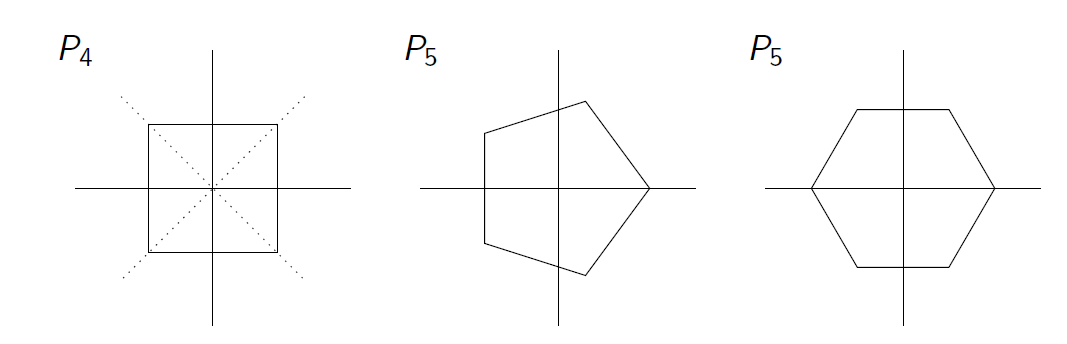
\includegraphics[scale=0.8]{Dihedral Groups.png}
\end{figure}\end{center}
$D_n<Isom(\mathbb{R}^2)$, $D_n=\{\Phi \in Isom(\mathbb{R}^2)|\Phi(P_n)=P_n\}$


\subsection{Some Properties of Group Operation}
\begin{proposition}[Proposition 3.1.1]
    Let $(G,*)$ be a group with identity $e\in G$, then
\end{proposition}
(1) if $g,h\in G$ and either $g*h=h$ or $h*g=h$, then $g=e$\\
(2) if $g,h\in G$ and $g*h=e$ then $g=h^{-1}$ and $h=g^{-1}$

\begin{corollary}[Corollary 3.1.2]
    $e^{-1}=e,\ (g^{-1})^{-1}=g,\ (g*h)^{-1}=h^{-1}*g^{-1}$
\end{corollary}


\subsection{Power of an Element}
We define $g^n$ recursively for $n \geq 0$ by setting $g^0 = e$ and for $n\geq 1$, we set $g^n = g^{n−1} * g$. For $n \leq 0$, we define $g^n = (g^{−1})^{-n}$.
\begin{proposition}[Proposition 3.1.5]
(1) $g^n*g^m=g^{n+m}$; (2) $(g^n)^m=g^{nm}$
\end{proposition}

\subsection{$(G\times H, \circledast)$: \underline{Direct Product} of $G$ and $H$}
$(G,*)$ a group $(H,\star)$ a group. Define an operation on $G\times H$, $\circledast$:\\
$$(h,k)\circledast(h',k')=(h*h',k*k')$$
\subsubsection{Proposition 3.1.7: $(G\times H, \circledast)$ is a group}
\begin{proposition}[Proposition 3.1.7]
$(G\times H, \circledast)$ is a group. The identity is $(e_G,e_H)$, inverse is $(g^{-1},h^{-1})$
\end{proposition}
usually written as
$$(h,k)(h',k')=(hh',kk')$$

\subsection{Subgroups and Cyclic Groups}

\subsubsection{Intersection of Subgroups is a Subgroup}
\begin{proposition}[Proposition 3.2.2]
Let $G$ be a group and suppose $\mathcal{H}$ is any collection of subgroups of $G$. Then $K=\cap_{H\in\mathcal{H}}H<G$ is a subgroup of $G$.
\end{proposition}


\subsubsection{Subgroup Generated by $A$: $\left\langle A\right\rangle$}
We define \textbf{Subgroup Generated by $A$:} $$\left\langle A\right\rangle=\cap_{H\in\mathcal{H}(A)}H$$
where $\mathcal{H}(A)$ is the set of all subgroups of $G$ containing the set $A$:
$$\mathcal{H}(A)=\{H<G|A\subset H \textit{ and }H \textit{ is a subgroup of } G \}$$


\subsubsection{Cyclic Group: group generated by an element}
A group $G$ is \underline{cyclic} if exists $g$ (an element), $\left\langle g\right\rangle=G$.

$g$ is called a \underline{generator} for $G$ in this case.

Easy to prove
$$G=\left\langle g\right\rangle =\{...g^{-2},g^{-1},e,g^1,g^2...\}$$



\subsubsection{Cyclic Subgroup}
If $A$ is a subgroup of $G$, and $A=\left\langle \{a\}\right\rangle=\left\langle a\right\rangle$. Then $A$ is the \underline{cyclic subgroup} generated by $a$: $A=\left\langle a\right\rangle\leq G$

$$\left\langle a\right\rangle =\{...a^{-2},a^{-1},e,a^1,a^2...\}$$


\subsubsection{Subgroups of a Cyclic Group must be Cyclic}
\begin{theorem}
A subgroup of a cyclic group is cyclic.
\end{theorem}
\begin{proof}
\quad\\
Let $G=\{a^n:n\in \mathbb{Z}\}$ be a cyclic group. Let $H\leq G$ be a subgroup.
\begin{enumerate}
    \item If $H=\{e\}$, then $H$ is cyclic.
    \item If $H\neq \{e\}$, then $a^n\in H$ for some $n>0$. Check $m$ be the minimal among all $n$.
    
    \underline{Claim}: $H=\left\langle a^m\right\rangle$

    \underline{Proof}: Clearly $\left\langle a^m\right\rangle\subset H$. $\forall a^n\in H$, $n=qm+r,0\leq r<m$. Then $a^r=a^n(a^m)^{-q}$. Since $m$ is the minimal positive integer s.t. $a^m\in H$, $r=0$. $\Rightarrow n=qm \Rightarrow a^n\in \left\langle a^m\right\rangle$. Hence $H=\left\langle a^m\right\rangle$ which is cyclic.
\end{enumerate}
\end{proof}
\begin{example}[Subgroups of $(\mathbb{Z},+)$]
\end{example}
$\mathbb{Z}$ is a cyclic group $\left\langle 1\right\rangle$. Its subgroups are $\left\langle n\right\rangle\leq \mathbb{Z}$ for some $n\geq 0$. (which is a multiplier of $n$. ($n \mathbb{Z}$))

$n=0,H=\{0\}; n=1,H=\mathbb{Z}; n=2,H=2 \mathbb{Z}$

\subsubsection{Theorem: $\left\langle a^v\right\rangle<\left\langle a^n\right\rangle$ $\Rightarrow$ $\left\langle a^v\right\rangle=\left\langle a^d\right\rangle, d=gcd(v,n), |\left\langle a^v\right\rangle|=\frac{n}{d}$}
\begin{theorem}
    Let $G$ be a cyclic group of order $n$. ($G=\{1,a,a^2,...,a^{n-1}\}$, where $a^n=1$.). Let $H= \left\langle a^v\right\rangle$ be a subgroup of $G$. Then $H$ is generated by $a^d$ (i.e. $H=\left\langle a^d\right\rangle$), $d=gcd(v,n)$ and $|H|=\frac{n}{d}$.
\end{theorem}
\begin{proof}
\quad\\
Let $H'=\left\langle a^d\right\rangle$, we need to show that $H=H'$. $d=gcd(v,n)=d|v \Rightarrow a^v\in \left\langle a^d\right\rangle \Rightarrow H\subset H'$.

While $d=sv+tn$ for some $s,t$. $\Rightarrow$ $a^d=(a^v)^s(a^n)^t$. Since $a^n=1$, $a^d=(a^v)^s \Rightarrow	H'\subset H$.

Hence, $H=H'=\left\langle a^v\right\rangle$. $H=\{1,a^d,a^{2d},...,a^{n-d}\}, |H|=\frac{n}{d}$
\end{proof}

\subsubsection{Corollary 3.2.4: $G$ is a cyclic group $\Rightarrow	$ $G$ is abelian}
\begin{corollary}[Corollary 3.2.4]
    If $G$ is a cyclic group (i.e. exits $g\in G$ s.t. $\left\langle g\right\rangle=G$), then $G$ is abelian (i.e. commutative).
\end{corollary}

\subsubsection{Equivalent properties of order of $g$: $|g|=|\left\langle g\right\rangle|<\infty$}
\begin{proposition}[Proposition 3.2.6]
    Let $G$ be a group for $g \in G$, the
    following are equivalent:
\end{proposition}
(i) $|g|<\infty$\\
(ii) $\exists n \neq m$ in $\mathbb{Z}$ so that $g^{n}=g^{m}$\\
(iii) $\exists n \in \mathbb{Z},\ n\neq 0$ so that $g^{n}=e$\\
(iv) $\exists n \in \mathbb{Z}_{+}$so that $g^{n}=e$\\
If $|g|<\infty$, then $|g|=$ smallest $n \in \mathbb{Z}_{+}$so that $g^{n}=e$, and $\langle g\rangle=\left\{e, g, g^{2}, \ldots, g^{n-1}\right\}=\left\{g^{n} \mid n=0, \ldots, n-1\right\}$

\subsubsection{$(\mathbb{Z},+)$ Theorem 3.2.9: $\left\langle a\right\rangle <\left\langle b\right\rangle$ if and only if $b|a$}
\begin{theorem}[Theorem 3.2.9]
    If $H < \mathbb{Z}$ is a subgroup, then either $H = \{ 0 \}$ , or else $H=\left\langle d\right\rangle$ , where $$d = \min \{ h \in H | h > 0 \}$$
    Consequently, $a \rightarrow \left\langle a\right\rangle$ defines a \textbf{bijection} from $N = \{ 0, 1, 2, . . . \}$ to the set of subgroups of $\mathbb{Z}$. Furthermore,
    for $a,b\in \mathbb{Z}_{+}$, we have $\left\langle a\right\rangle <\left\langle b\right\rangle$ if and only if $b|a$.
\end{theorem}

\subsubsection{$(\mathbb{Z}_n,+)$ Theorem 3.2.10: $\left\langle [d]\right\rangle<\left\langle [d']\right\rangle$ if and only if $d'|d$}
\begin{theorem}[Theorem 3.2.10]
For any $n \geq 2$, if $H <\mathbb{Z}_n$ is a subgroup, then there is a positive divisor $d$ of $n$ so that $$H=\left\langle [d]\right\rangle$$
Furthermore, this defines a bijection between divisors of $H$ and subgroups of $\mathbb{Z}_n$. Furthermore, if $d, d'> 0$ are two divisors of $n$, then $\left\langle [d]\right\rangle<\left\langle [d']\right\rangle$ if and only if $d'|d$.
\end{theorem}
If $H=\left\langle [d]\right\rangle$ is a subgroup of $H$, then $[n]\in H$, so $d|n$. And $|H|=|\left\langle [d]\right\rangle|=\frac{n}{d}$, so $|H|\vert d$

\subsubsection{Subgroup Lattice}
The set of all subgroups of a group of G, together with the data of which subgroups contain which others is called the \textbf{subgroup lattice}. We often picture the subgroup lattice in a diagram with the entire group at the top, the trivial subgroup $\{ e \} $ at the bottom, and the intermediate subgroups in the middle, with lines drawn from subgroups up to larger groups.
\begin{center}\begin{figure}[htbp]
    \centering
    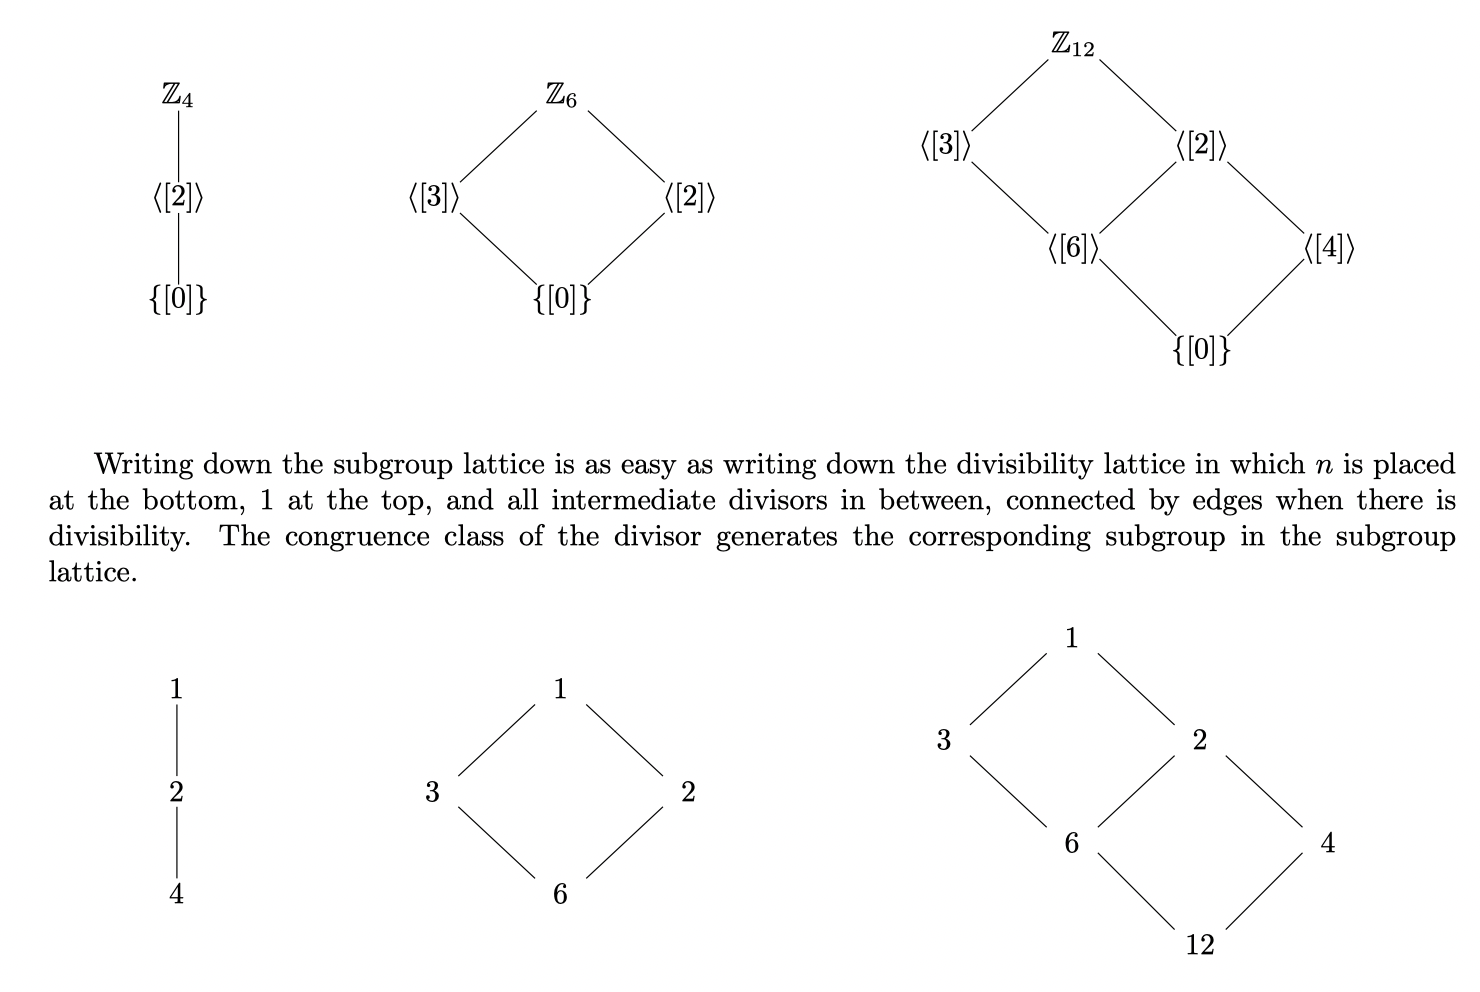
\includegraphics[scale=0.4]{lec1301.png}
    \caption{}
    \label{}
\end{figure}\end{center}







\subsection{Homomorphism}
\subsubsection{Definition: Homomorphism}
\begin{definition}
If $(G,*)$ and $(H,\circ)$ are groups, then a function $f:G \rightarrow	H$ is a \textbf{homomorphism} if $$f(x*y)=f(x)\circ f(y),\ \forall x,y\in G$$
If $f$ is also a bijection, then $f$ is called an \textbf{isomorphism}.
\end{definition}

\begin{example}
\end{example}
\begin{enumerate}
    \item $\phi: (\mathbb{R},+) \rightarrow	(\mathbb{R}^*,x)\quad \phi(x)=2^x$. Then
    $$\phi(x+y)=2^{x+y}=2^x2^y=\phi(x)\phi(y)$$ $\phi$ is a homonorphism.
    \item $\phi: G \rightarrow	G\quad \phi(g)=g^{-1}$. Then
    $$\phi(gh)=(gh)^{-1}=h^{-1}g^{-1}=\phi(h)\phi(g)$$ $\phi$ is not a homonorphism in general; but it is homomorpgism if it is abelian.
\end{enumerate}

\subsubsection{Properties of Homomorphism}
\begin{theorem}
    Let $\phi$ be a homomorphism of a group $G$ into a group $G'$, then
\end{theorem}
\begin{enumerate}
    \item if $e\in G$ is an identity in $G$, then $\phi(e)\in G'$ is the identity in $G'$.
    \item if $a\in G$ has inverse $a'\in G$, then $\phi(a)\in G'$ has inverse $\phi(a')\in G'$.
    \item if $H\leq G$ is a subgroup of $G$, then the image $\phi(H)=\{\phi(h):h\in G\}\leq G'$ is a subgroup of $G'$.
    \item if $K'\leq G'$ then the inverse image $\phi^{-1}(K')=\{x\in G:\phi(x)\in K'\}\leq G$.
\end{enumerate}

\subsubsection{Kernel of Homomorphism}
\begin{definition}
    Let $\phi: G \rightarrow G'$ be a homomorphism of groups. The subgroup $\phi^{-1}(e')=\{x\in G:\phi(x)=e'\}$ is the kernel of $\phi$, denoted by $Ker (\phi)$.
    $$Ker (\phi) \stackrel{def}{=} \phi^{-1}(e')=\{x\in G:\phi(x)=e'\}$$
\end{definition}

\begin{theorem}
Let $\phi: G \rightarrow G'$ be a homomorphism. $H=Ker\phi$, then for all $a\in G$, $\phi^{-1}[\phi(a)]=\{x\in G:\phi(x)=\phi(a)\}$ is the left coset $aH$ of $H$, and is also the right coset $Ha$ of $H$.
$$aH=Ha=\{x\in G:\phi(x)=\phi(a)\}$$
\end{theorem}
\begin{proof}
\begin{equation}
    \begin{aligned}
        &\phi(x)=\phi(a)\\
        \Leftrightarrow\quad	&\phi(x)\phi(a)^{-1}=e'\\
        \Leftrightarrow\quad	&\phi(x)\phi(a^{-1})=e'\\
        \Leftrightarrow\quad	&\phi(xa^{-1})=e'\\
        \Leftrightarrow\quad	&xa^{-1}\in H\\
        \Leftrightarrow\quad	&x\in Ha\\
    \end{aligned}
    \nonumber
\end{equation}
Similarity, we can prove $x\in aH$.
\end{proof}

\subsection{Isomorphism}
\subsubsection{Definition: Isomorphism}
\begin{definition}
    We say that $G$ and $H$ are \textbf{isomorphic} if exists an \textbf{isomorphism} $f$, denoted by $G\cong H$. (since $f$ is bijection, $G\cong H\Leftrightarrow H\cong G$)
\end{definition}
\begin{corollary}
A homomorphism is isomorphism if and only if $Ker(\phi)=\{e\}$.
\end{corollary}

Isomophic means these two pathes are the same.
\begin{equation}
    \begin{aligned}
        G\times G& \stackrel{*}{\longrightarrow} & G &\stackrel{f}{\longrightarrow}& H\\
        G\times G& \stackrel{(f,f)}{\longrightarrow} &H\times H & \stackrel{\circ}{\longrightarrow}& H\\
    \end{aligned}
    \nonumber
\end{equation}

\begin{example}
    $(\mathbb{Z}_2,+)$, $(\{-1,1\},\times)$ and $\phi: 0 \rightarrow 1;\ 1 \rightarrow -1$.
    \begin{equation}
        \begin{aligned}
            \phi(0+0)=1=\phi(0)\times\phi(0)\\
            \phi(0+1)=-1=\phi(0)\times\phi(1)\\
            \phi(1+1)=1=\phi(1)\times\phi(1)\\
        \end{aligned}
        \nonumber
    \end{equation}
\end{example}


\subsubsection{Theorem: $\left\{\begin{matrix}
    \sigma: G \rightarrow G'\text{ injective}\\
    \sigma(xy)=\sigma(x)\sigma(y)\ \forall x,y\in G
\end{matrix}\right. \Rightarrow	\sigma(G)\leq G'$, $G$ is isomorphic to $\sigma(G)$}
\begin{theorem}
Let $\sigma: G \rightarrow G'$ be an injective map s.t. $$\sigma (xy)=\sigma(x)\sigma(y),\ \forall x,y\in G$$
Then the image $\sigma(G)=\{\sigma(x):x\in G\}$ is a subgroup of $G'$ that is isomorphic to $G$.
\end{theorem}
\begin{proof}
\quad\\
\begin{enumerate}
    \item Closed: $\forall a=\sigma(x),b=\sigma(y)\in \sigma(G)$, then $ab=\sigma(x)\sigma(y)=\sigma(xy)\in \sigma(G)$.
    \item Identity: $\sigma(e)\in \sigma(G)$ is an identity for $\sigma(G)$: $\sigma(e)\sigma(x)=\sigma(ex)=\sigma(x)=\sigma(xe)=\sigma(x)\sigma(e)$
    \item Inverse: $\sigma(x^{-1})$ is an inverse in $\sigma(G)$ for $\sigma(x)$: $\sigma(x^{-1})\sigma(x)=\sigma(e)=\sigma(x)\sigma(x^{-1})$
\end{enumerate}
\end{proof}

\subsubsection{Cayley Theorem: $G$ is isomorphic to a subgroup of $S_G$}
\begin{theorem}[Cayley Theorem]
Let $G$ be a group and $S_G$ is the symmetric group of $G$ (the group of all permutation of $G$: $S_G=\{\text{Bijection } \sigma: G \rightarrow G\}$)
Then $G$ is isomorphic to a subgroup of $S_G$.
\end{theorem}
\begin{proof}
\quad\\
Set a bijection $\phi: G \rightarrow S_G$ such that $\phi(g)=\lambda_g, \forall g\in G$, where $\lambda_g$ is a permutation $\lambda_g: x \rightarrow gx$.

Claim: $\lambda_g\in S_G$ (i.e. $\lambda_g$ is a permutation of $G$, a \underline{bijection} $G \rightarrow	G$).
\begin{enumerate}
    \item $\lambda_g: G \rightarrow G$ is \underline{injective}
    \begin{equation}
        \begin{aligned}
            \lambda_g(x)&=\lambda_g(y)\\
            \Leftrightarrow	gx&=gy\\
            \Leftrightarrow	x&=y\\
        \end{aligned}
        \nonumber
    \end{equation}
    \item $\lambda_g: G \rightarrow G$ is \underline{surjective}. Let $y\in G$
    \begin{equation}
        \begin{aligned}
            \lambda_g(x)&=y\\
            \Leftrightarrow	gx&=y\\
            \Leftrightarrow	x&=g^{-1}y\\
        \end{aligned}
        \nonumber
    \end{equation}
\end{enumerate}


Claim: $\phi(x)\phi(y)=\phi(xy)$
\begin{equation}
    \begin{aligned}
        \phi(x)\phi(y)=\lambda_x\circ\lambda_y\\
        (\lambda_x\circ\lambda_y)(z)=\lambda_x(yz)=xyz=\lambda_{xy}(z),\ \forall z\in G\\
        \Rightarrow	\phi(x)\phi(y)=\phi(xy)
    \end{aligned}
    \nonumber
\end{equation}

According to previous theorem, $\phi(G)\leq G$ and $G$ is isomorphic to $\phi(G)$.

\end{proof}













\subsection{Coset and Order}
\begin{definition}
If $H$ is a subgroup of a group $G$ and $a\in G$, then $aH=\{ah|h\in H\}\leq G$ is called \underline{left coset} of H.
\end{definition}
\begin{theorem}
Let $H\leq G$, $a,b\in G$,
\begin{enumerate}
    \item $aH=bH$ if and only if $a^{-1}b\in H$
    \item $aH\cap bH=\emptyset$ or $aH=bH$
    \item $|aH|=|H|\ \forall a\in G$
\end{enumerate}
\end{theorem}
\begin{proof}
    \quad

    \begin{enumerate}
        \item Assume that $aH\cap bH\neq \emptyset$ and let $ah=bk\in aH\cap bH$ with $h,k\in H$.

        $ah=bk\Leftrightarrow h=a^{-1}bk \Leftrightarrow a^{-1}b=hk^{-1}\in H$, thus $a^{-1}b\in H$.
        \item When $aH\cap bH\neq \emptyset$ $\exists k_1,h\in H$ such that $ak_1=bh\in bH$. Then $\forall k_2\in H$ $a=bhk_1^{-1} \Rightarrow ak_2=bhk_1^{-1}k_2$ wheere $hk_1^{-1}k_2\in H$ so $ak_2\in bH,\ \forall k_2\in H$.
        \item $x \rightarrow ax$ is bijection $\Rightarrow |aH|=|H|$.
    \end{enumerate}
\end{proof}

\begin{claim}
Coset can generate a partition of group:
$$G=a_1H\cup a_2H\cup \cdots \cup a_rH$$
\end{claim}

\subsubsection{index of a subgroup}
\begin{definition}
    Let H be a subgroup of a group G. \underline{The number of left cosets of H in G} is the \textbf{index}.
\end{definition}
\textbf{Note:} Since $|aH|=|H|\ \forall a\in G$, the index of a subgroup is the number of subgroups which have order $|H|$.






\subsubsection{Lagrange Theorem: Order of subgroup divides the order of group}
\begin{theorem}[Lagrange Theorem]
    Let $H\leq G$ be a subgroup of finite group $G$. Then the order $|H|$ divides the order $|G|$.
\end{theorem}
\begin{proof}
\quad\\
Give a partition
\begin{equation}
    \begin{aligned}
        G&=a_1H\cup a_2H\cup \cdots \cup a_rH\\
        |G|&=|a_1H|+ |a_2H|+ \cdots + |a_rH|\\
        &=r|H|\rightarrow |H|\bigg||G|
    \end{aligned}
    \nonumber
\end{equation}
\end{proof}

\subsubsection{Theoerm: Order of element $a\in G =|\left\langle a\right\rangle|$ divides $|G|$}
\begin{theorem}[Order of element/cyclic subgroup]
For $a\in G$, the order of $a$ (the smallest $m$ such that $a^m=e$) divides $|G|$. The order of $a$ is the order of cyclic subgroup $\left\langle a\right\rangle$ with generator $a$.
\end{theorem}

\begin{proof}
\quad\\
For $a\in G$, $H=\{a^n,n\in \mathbb{Z}\}\leq G$. $H$ is the size of $m$. With lagrange theorm, $|H|=m\bigg||G|$
\end{proof}

\begin{corollary}
Every group of prime order is cyclic.
\end{corollary}

\subsubsection{Theorem: Order $n$ cyclic group is isomorphic to $(\mathbb{Z}_n,+_n)$}
\begin{theorem}
    Let $G$ be a cyclic group with generator $a$. If the order of $G$ is infinite, then G is isomorphic to $(\mathbb{Z},+)$. If $G$ has finite order $n$, then $G$ is isomorphic to $(\mathbb{Z}_n,+_n)$.
\end{theorem}


\subsection{Direct Products}
\subsubsection{Cartesian product}
Let $G_1,G_2,...,G_n$ be $n$ groups. Let $G=G_1\times G_2\times\cdots\times G_n$ be the Cartesian product.

For $g\in G$, $g=(g_1,...,g_n)$, $g_i\in G_i$.

\begin{theorem}
Then $(G,*)$ becomes a group with operation $*$ defined as
$$a*b=(a_1,...,a_n)*(b_1,...,b_n)=(a_1b_2,...,a_nb_n)\quad a,b\in G$$
\end{theorem}
\begin{proof}
    \quad

\begin{enumerate}[(1)]
    \item Binary operation $*:G\times G \rightarrow	G$.
    \item $*$ is associative: $$(a*b)*c=a*(b*c)=(a_1b_1c_1,...,a_nb_nc_n)$$
    \item Identity: $e=(e_1,...,e_n)\in G$ $$e*a=a=a*e$$
    \item Inverse: $a^{-1}=(a_1^{-1},...,a_n^{-1})\in G$ $$a*a^{-1}=a^{-1}*a=e$$
\end{enumerate}
\end{proof}

\subsubsection{Theorem: $\mathbb{Z}_m\times \mathbb{Z}_n$ is cyclic and is isomorphic to $\mathbb{Z}_{mn}$ $\Leftrightarrow gcd(m,n)=1$}
\begin{theorem}
The group $\mathbb{Z}_m\times \mathbb{Z}_n$ is cyclic and is isomorphic to $\mathbb{Z}_{mn}$ if and only if $gcd(m,n)=1$.
\end{theorem}
\begin{proof}
\quad\\
\textbf{Claim:} $(1,1)$ generate $\mathbb{Z}_m\times \mathbb{Z}_n$

$k(1,1)=(k,k)=(0,0)$ if and only if $m|k$ and $n|k$. The smallest such $k$ is $k=lcm(m,n)=mn$. Hence, $\mathbb{Z}_m\times \mathbb{Z}_n$ is a cyclic group with order $mn$. Then $\mathbb{Z}_m\times \mathbb{Z}_n$ is isomorphic to $\mathbb{Z}_{mn}$.

We can define an isomorphism $$\phi:\mathbb{Z}_m\times \mathbb{Z}_n \rightarrow \mathbb{Z}_{mn}$$ and its inverse $$\psi: \mathbb{Z}_{mn} \rightarrow \mathbb{Z}_m\times \mathbb{Z}_n$$
Since $\mathbb{Z}_{mn}\left\langle 1\right\rangle$, $\mathbb{Z}_m\times \mathbb{Z}_n=\left\langle (1,1)\right\rangle$, we can write $$\psi(x\text{ mod }mn)=(x\text{ mod }m,x\text{ mod }n)$$
$\psi$ is well-defined.

To describe $\phi:\mathbb{Z}_m\times \mathbb{Z}_n \rightarrow \mathbb{Z}_{mn}$ at $1=sm+tn$ and let $$\phi(a\text{ mod }m,b\text{ mod }n)=(atn+bsm\text{ mod }mn)$$
\begin{equation}
    \begin{aligned}
        \psi(atn+bsm\text{ mod }mn)&=(atn+bsm\text{ mod }m,atn+bsm\text{ mod }n)\\
        &=(atn\text{ mod }m,bsm\text{ mod }n)\\
        &=(a(1-sm)\text{ mod }m,b(1-tn)\text{ mod }n)\\
        &=(a\text{ mod }m,b\text{ mod }n)
    \end{aligned}
    \nonumber
\end{equation}
Hence $\psi$ is the inverse of $\phi$.
\end{proof}



\begin{corollary}
    The group $\prod_{i=1}^n \mathbb{Z}_{m_i}$ is cyclic and is isomorphic to $\mathbb{Z}_{m_1m_2\cdots m_n}$ if and only if the numbers $m_i$ for $i=1,...,n$ are such that the gcd of any two of them is $1$.
\end{corollary}
\begin{example}
If $n$ is written as a product of powers of distinct prime numbers, as it $$n=(p_1)^{n_1}(p_2)^{n_2}\cdots(p_r)^{n_r}$$
then $\mathbb{Z}_n$ is isomorphic to $$\mathbb{Z}_{(p_1)^{n_1}}\times \mathbb{Z}_{(p_2)^{n_2}}\times \cdots\times \mathbb{Z}_{(p_r)^{n_r}}$$
\end{example}

\subsubsection{Finitely Generated Abelian Groups}
\begin{theorem}[Primary Factor Version of the Fundamental Theorem of Finitely Generated Abelian Groups]
Every finitely generated abelian group $G$ is isomorphic to a direct product of cyclic groups in the form $$\mathbb{Z}_{(p_1)^{r_1}}\times \mathbb{Z}_{(p_2)^{r_2}}\times \cdots\times \mathbb{Z}_{(p_n)^{r_n}}\times \mathbb{Z}\times \mathbb{Z}\times \cdots \times \mathbb{Z}$$
where the $p_i$ are primes, not necessarily distinct, and the $r_i$ are positive integers. The number of factors of $\mathbb{Z}$ and the prime powers $(p_i)^{r_i}$ are unique.
\end{theorem}
\begin{enumerate}[$\bullet$]
    \item $\mathbb{Z}_{mn}\simeq \mathbb{Z}_m\times \mathbb{Z}_n$ if $gcd(m,n)=1$.
    \item Abelian $\Leftrightarrow$ $\mathbb{Z}_m\times \mathbb{Z}_n=\mathbb{Z}_n\times \mathbb{Z}_m$
\end{enumerate}



\begin{example}
Find all abelian group of order 16
\end{example}
5 nonisomorphic abelian group.
\begin{equation}
    \begin{aligned}
        \left\{\begin{matrix}
            \mathbb{Z}_{16}&&&\\
            \mathbb{Z}_8&\times \mathbb{Z}_2&&\\
            \mathbb{Z}_4&\times\mathbb{Z}_4&&\\
            \mathbb{Z}_4&\times \mathbb{Z}_2&\times \mathbb{Z}_2&\\
            \mathbb{Z}_2&\times \mathbb{Z}_2&\times \mathbb{Z}_2&\times \mathbb{Z}_2
        \end{matrix}\right.
    \end{aligned}
    \nonumber
\end{equation}
\begin{example}
\end{example}
\begin{equation}
    \begin{aligned}
        \mathbb{Z}_{6}\times \mathbb{Z}_{40}\times \mathbb{Z}_{49}&\simeq \mathbb{Z}_2\times \mathbb{Z}_3\times \mathbb{Z}_5\times \mathbb{Z}_8\times \mathbb{Z}_{49}\\
        \mathbb{Z}_{210}\times \mathbb{Z}_{56}&\simeq \mathbb{Z}_3\times \mathbb{Z}_7\times \mathbb{Z}_2\times \mathbb{Z}_5\times \mathbb{Z}_{7}\times \mathbb{Z}_{8}\\
    \end{aligned}
    \nonumber
\end{equation}

\subsection{Factor Group}
\subsubsection{Definition}
\begin{definition}
    Let $\phi: G \rightarrow G'$ be a homomorphism of groups with \underline{kernel $H$}. Then the cosets of $H$ form
    a \textbf{factor group}, $G/H=\{aH:a\in G\}$. where $(aH)(bH) = (ab)H$.
\end{definition}
Also, the map $\mu: G/H \rightarrow \phi[G]$
    defined by $\mu(aH) = \phi(a)$ is an isomorphism. Both coset multiplication and $\mu$ are well
    defined, independent of the choices $a$ and $b$ from the cosets.


\subsubsection{Normal Subgroup}
\begin{definition}
    A subgroup $H\leq G$ is \textbf{normal} if its left and right cosets coincide, that is, if $$aH=Ha,\quad \forall a\in G$$
    Notation: $H \lhd G$
\end{definition}
\textbf{Note} that all subgroups of abelian groups are normal.
\begin{corollary}
    $ker\phi$ is a normal subgroup: $ker\phi \lhd G$ for all homonorphisms.
\end{corollary}

\subsubsection{Well-defined Left Cosets Multiplication $\Leftrightarrow$ Normal Subgroup}
\begin{theorem}
    Let $H$ be a subgroup of a group $G$. Then left coset multiplication is well defined by the equation
    $$(aH)(bH) = (ab)H$$
    if and only if $H \lhd G$ ($H$ is a normal subgroup of $G$).

    i.e. '$x\in aH$ and $y\in bH$ $\Rightarrow$ $xy\in abH$' \underline{if and only if} '$aH=Ha,\quad \forall a\in G$'
\end{theorem}
\begin{proof}
    \quad

\begin{enumerate}[$\bullet$]
    \item "$\Rightarrow$": $\forall x\in aH$, $a^{-1}\in a^{-1}H$ $\Rightarrow$ $xa^{-1}\in H \Leftrightarrow x\in Ha \Rightarrow aH\subset Ha$;
    
    \quad Similarly $a^{-1}H\subset Ha^{-1} \Leftrightarrow	Ha\subset aH$ $\Rightarrow	aH=Ha$
    \item "$\Leftarrow$": Let $x\in aH$, $y\in bH$. Say $x=ah_1, y=bh_2$
    \begin{equation}
        \begin{aligned}
            xy&=(ah_1)(bh_2)\\
            &=a(h_1 b)h_2\\
            &=a(b h_3)h_2 \quad \text{(Since $bH=Hb$)}\\
            &=(ab)(h_3 h_2)\in abH
        \end{aligned}
        \nonumber
    \end{equation}
\end{enumerate}
\end{proof}

\begin{definition}
    The group $G/H=\{aH:a\in G\}$ with $(aH)(bH)=abH$ is the factor group (or quotient group) of
    $G$ by $H$.
\end{definition}
\begin{corollary}
    Let $H\lhd  G$ be a \textbf{normal subgroup} of $G$. Then the cosets of $H$ form a group $G/H=\{aH:a\in G\}$ under the
    binary operation $(aH)(bH) = (ab)H$.
\end{corollary}
\begin{proof}
\quad

\begin{enumerate}[$(1)$]
    \item $*$ is associative.
    \item $G/H$ has an identity $H$. $$H*aH=aH*H=aH$$
    \item $aH\in G/H$ has inverse $a^{-1}H$
\end{enumerate}
\end{proof}

\subsubsection{The Fundamental Homomorphism Theorem}
\begin{theorem}
Let $H \lhd G$ be a normal subgroup of $G$. Define $\gamma: G \rightarrow G/H$, $\gamma(x)=xH$. Then $\gamma$ is a surjective homomorphism with $ker \gamma=H$.
\end{theorem}
\begin{proof}
    \quad
\begin{enumerate}
    \item $\gamma$ is surjective homomorphism: $\gamma(ab)=abH=(aH)(bH)=\gamma(a)\gamma(b)$
    \item $ker\gamma=H$: The identity in $G/H$ is the coset $H$.
    \begin{equation}
        \begin{aligned}
            ker\gamma=\gamma^{-1}(H)&=\{a\in G: \gamma(a)=aH=H\}\\
            &=\{a\in G: a\in H\}=H
        \end{aligned}
        \nonumber
    \end{equation}
\end{enumerate}
\end{proof}

\begin{theorem}[The Fundamental Homomorphism Theorem]
    Let $\phi: G \rightarrow G'$ be a group
    homomorphism with kernel $H$.
    
    Then $\phi[G]$ is a group, and $\mu: G/H \rightarrow \phi[G]$ given by $\mu(gH)=\phi(g)$ is an \underline{isomorphism}.
    
    If $\gamma:G \rightarrow G/H$ is the homomorphism given by $\gamma(g) = gH$, then $\phi(g) = \mu\gamma(g)$ for each $g\in G$.
    
\end{theorem}





\section{Ring $(R,+,\cdot)$: $+$ is associative, commutative, identity, inverse $\in R$; $\cdot$ is associative, distributes over $+$}
\begin{definition}
    A ring is a nonempty set with two operations, called addition and multiplication, $(R,+,\cdot)$ such that
\end{definition}
(1): $(R,+)$ is an ablian group: i.e. $+$ is associatve and commucative. $0,-a\in R$\\
(2): $\cdot$ is associative.\\
(3): $\cdot$ distributes over $+$: $\forall a,b,c\in R$, $a\cdot(b+c)=a\cdot b+a\cdot c$ and $(b+c)\cdot a=b\cdot a+c\cdot a$
\subsection{Commutative ring: ring's $\cdot$ is commutative}
If "$\cdot$" is commutative, we call $(R, +, \cdot)$ a commutative ring.
\subsection{Ring with 1: exists multiplication identity $1\in R$}
If there exists an element $1\in R\backslash \{0\}$ such that $a1=1a=a,\ \forall a\in R$,then we say that $R$ is a ring with 1.

\subsection{Field $\mathbb{F}$ is a commutative ring with 1; $\mathbb{F}[x]$ is also a commutative ring with 1}
Field $(\mathbb{F}, +, \cdot)$ (close, associative, commutative, distributive(M over A), identity $\&$ inverse(M,A))\\
Proposition 2.3.2: Polynomial ring (close, associative, commutative, distributive(M over A), identity(M,A), inverse(only A))

\subsection{$S\subset R$: Subring (closed under $+$ and $\cdot$; addictive inverse $-a\in S$)}
\subsubsection{Proposition 2.6.27: $(S,+,\cdot)$ is a ring}
\begin{proposition}[Proposition 2.6.27]
    If $S\subset R$ is a subring, then $+,\cdot$ make $S$ into a ring.
\end{proposition}

































































































\begin{thebibliography}{1}
    \bibitem{Long2015Fully}
    Christopher J Leininger  \newblock Introduction to Abstract Algebra
    (Draft)  2017.

    \bibitem{Long2015Fully}
    Fraleigh, J. B. (2003). A first course in abstract algebra. Pearson Education India.
\end{thebibliography}


\end{document}
\bibliography{reference}
\bibliographystyle{unsrt}